% !TeX root = OVATiK.tex
\documentclass[11pt,a4paper]{article}
%\documentclass[a4paper,12pt, draft]{article}
\documentclass[a4paper,12pt]{article}

%%% Работа с русским языком
\usepackage{cmap}					% поиск в PDF
\usepackage{mathtext} 				% русские буквы в формулах
\usepackage[T2A]{fontenc}			% кодировка
\usepackage[utf8]{inputenc}			% кодировка исходного текста
\usepackage[english,russian]{babel}	% локализация и переносы
\usepackage{indentfirst}            % красная строка в первом абзаце
\frenchspacing                      % равные пробелы между словами и предложениями

%%% Дополнительная работа с математикой
\usepackage{amsmath,amsfonts,amssymb,amsthm,mathtools} % пакеты AMS
\usepackage{icomma}                                    % "Умная" запятая

%%% Свои символы и команды
\usepackage{centernot} % центрированное зачеркивание символа
\usepackage{stmaryrd}  % некоторые спецсимволы

\renewcommand{\epsilon}{\ensuremath{\varepsilon}}
\renewcommand{\phi}{\ensuremath{\varphi}}
\renewcommand{\kappa}{\ensuremath{\varkappa}}
\renewcommand{\le}{\ensuremath{\leqslant}}
\renewcommand{\leq}{\ensuremath{\leqslant}}
\renewcommand{\ge}{\ensuremath{\geqslant}}
\renewcommand{\geq}{\ensuremath{\geqslant}}
\renewcommand{\emptyset}{\ensuremath{\varnothing}}

\DeclareMathOperator{\sgn}{sgn}
\DeclareMathOperator{\ke}{Ker}
\DeclareMathOperator{\im}{Im}
\DeclareMathOperator{\re}{Re}

\newcommand{\N}{\mathbb{N}}
\newcommand{\Z}{\mathbb{Z}}
\newcommand{\Q}{\mathbb{Q}}
\newcommand{\R}{\mathbb{R}}
\newcommand{\Cm}{\mathbb{C}}
\newcommand{\F}{\mathbb{F}}
\newcommand{\id}{\mathrm{id}}
\newcommand{\imp}[2]{
	(#1\,\,$\ra$\,\,#2)\,\,
}
\newcommand{\System}[1]{
	\left\{\begin{aligned}#1\end{aligned}\right.
}
\newcommand{\Root}[2]{
	\left\{\!\sqrt[#1]{#2}\right\}
}
\newcommand{\RR}{\R}
\newcommand{\NN}{\N}
\renewcommand{\subseteq}{\subset}
\newcommand{\sub}{\subset}
\newcommand{\sconstr}{\;\vert\;}
\newcommand{\thus}{\implies}

\newcommand{\defeq}{\vcentcolon= }
\newcommand{\defev}{\stackrel{\Delta}{\Longleftrightarrow}}
\newcommand{\deriv}[3][1]{%
	\ifthenelse{#1>1}{%
		\frac{\dlta^{#1} {#2}}{\dlta {#3}^{#1}}
	}{%
		\frac{\dlta {#2}}{\dlta {#3}}
	}%
}

\renewcommand\labelitemi{$\triangleright$}

\let\bs\backslash
\let\lra\Leftrightarrow
\let\ra\Rightarrow
\let\la\Leftarrow
\let\emb\hookrightarrow

%%% Перенос знаков в формулах (по Львовскому)
\newcommand{\hm}[1]{#1\nobreak\discretionary{}{\hbox{$\mathsurround=0pt #1$}}{}}

%%% Работа с картинками
\usepackage{graphicx}    % Для вставки рисунков
\setlength\fboxsep{3pt}  % Отступ рамки \fbox{} от рисунка
\setlength\fboxrule{1pt} % Толщина линий рамки \fbox{}
\usepackage{wrapfig}     % Обтекание рисунков текстом

%%% Работа с таблицами
\usepackage{array,tabularx,tabulary,booktabs} % Дополнительная работа с таблицами
\usepackage{longtable}                        % Длинные таблицы
\usepackage{multirow}                         % Слияние строк в таблице

%%% Теоремы
\theoremstyle{plain}
\newtheorem{theorem}{Теорема}[section]
\newtheorem{lemma}{Лемма}[section]
\newtheorem{proposition}{Утверждение}[section]
\newtheorem*{exercise}{Упражнение}
\newtheorem*{problem}{Задача}

\theoremstyle{definition}
\newtheorem{definition}{Определение}[section]
\newtheorem*{corollary}{Следствие}
\newtheorem*{note}{Замечание}
\newtheorem*{reminder}{Напоминание}
\newtheorem*{example}{Пример}

\theoremstyle{remark}
\newtheorem*{solution}{Решение}

%%% Оформление страницы
\usepackage{extsizes}     % Возможность сделать 14-й шрифт
\usepackage{geometry}     % Простой способ задавать поля
\usepackage{setspace}     % Интерлиньяж
\usepackage{enumitem}     % Настройка окружений itemize и enumerate
\setlist{leftmargin=25pt} % Отступы в itemize и enumerate

\geometry{top=25mm}    % Поля сверху страницы
\geometry{bottom=30mm} % Поля снизу страницы
\geometry{left=20mm}   % Поля слева страницы
\geometry{right=20mm}  % Поля справа страницы

\setlength\parindent{15pt}        % Устанавливает длину красной строки 15pt
\linespread{1.3}                  % Коэффициент межстрочного интервала
%\setlength{\parskip}{0.5em}      % Вертикальный интервал между абзацами
%\setcounter{secnumdepth}{0}      % Отключение нумерации разделов
%\setcounter{section}{-1}         % Нумерация секций с нуля
\usepackage{multicol}			  % Для текста в нескольких колонках
\usepackage{soulutf8}             % Модификаторы начертания
\mathtoolsset{showonlyrefs=true} % показывать номера формул только у тех, у которых есть ссылки по eqref
%%% Содержаниие
\usepackage{tocloft}
\tocloftpagestyle{main}
%\setlength{\cftsecnumwidth}{2.3em}
%\renewcommand{\cftsecdotsep}{1}
%\renewcommand{\cftsecpresnum}{\hfill}
%\renewcommand{\cftsecaftersnum}{\quad}

%%% Шаблонная информация для титульного листа
\newcommand{\CourseName}{Математический анализ}
\newcommand{\FullCourseNameFirstPart}{\so{Введение в математический анализ}}
\newcommand{\SemesterNumber}{I}
\newcommand{\LecturerInitials}{Гусев Николай Анатольевич}
\newcommand{\CourseDate}{осень 2022}
\newcommand{\AuthorInitials}{Копанов Антон}
\newcommand{\AuthorInitialssecond}{Клищ Данил}
\newcommand{\VKLink}{https://vk.com/notnako}
\newcommand{\GithubLink}{https://github.com/MIPT-Group/Lectures_Tex_Club}
\newcommand{\VKLinksecond}{https://vk.com/dan.klishch}

%%% Колонтитулы
\usepackage{titleps}
\newpagestyle{main}{
	\setheadrule{0.4pt}
	\sethead{\CourseName}{}{\hyperlink{intro}{\;Назад к содержанию}}
	\setfootrule{0.4pt}                       
	\setfoot{ФПМИ МФТИ, \CourseDate}{}{\thepage} 
}
\pagestyle{main}  

%%% Нумерация уравнений
\makeatletter
\def\eqref{\@ifstar\@eqref\@@eqref}
\def\@eqref#1{\textup{\tagform@{\ref*{#1}}}}
\def\@@eqref#1{\textup{\tagform@{\ref{#1}}}}
\makeatother                      % \eqref* без гиперссылки
\numberwithin{equation}{section}  % Нумерация вида (номер_секции).(номер_уравнения)
\mathtoolsset{showonlyrefs= true} % Номера только у формул с \eqref{} в тексте.

%%% Гиперссылки
\usepackage{hyperref}
\usepackage[usenames,dvipsnames,svgnames,table,rgb]{xcolor}
\hypersetup{
	unicode=true,            % русские буквы в раздела PDF
	colorlinks=true,       	 % Цветные ссылки вместо ссылок в рамках
	linkcolor=black!15!blue, % Внутренние ссылки
	citecolor=green,         % Ссылки на библиографию
	filecolor=magenta,       % Ссылки на файлы
	urlcolor=NavyBlue,       % Ссылки на URL
}

%%% Графика
\usepackage{tikz}        % Графический пакет tikz
\usepackage{tikz-cd}     % Коммутативные диаграммы
\usepackage{tkz-euclide} % Геометрия
\usepackage{stackengine} % Многострочные тексты в картинках
\usetikzlibrary{angles, babel, quotes}

\begin{document}
    %%% Всю шаблонную информацию можно менять тут
\newcommand{\FullCourseNameFirstPart}{\so{ТЕОРИЯ ГРУПП}}
\newcommand{\SemesterNumber}{III}
\newcommand{\LecturerInitials}{Богданов Илья Игоревич}
\newcommand{\AutherInitials}{Даниил Дрябин}
\newcommand{\VKLink}{https://vk.com/ax_equals_b}
\newcommand{\GithubLink}{https://github.com/daniild71r/lectures_tex_club}

\begin{titlepage}
	\clearpage\thispagestyle{empty}
	\centering
	
	%\textit{Федеральное государственное автономное учреждение \\
	%	высшего профессионального образования}
	%\vspace{0.5ex}
	
	%\textbf{Московский Физико-Технический Институт \\ КЛУБ ТЕХА ЛЕКЦИЙ}
	\textbf{Московский физико-технический институт \\ Физтех-школа прикладной математики и информатики}
	\vspace{20ex}
	\vspace{13ex}
	
	{\textbf{\FullCourseNameFirstPart}}
	
	\SemesterNumber\ СЕМЕСТР  
	\vspace{1ex}
	
	Лектор: \textit{\LecturerInitials}
	
	\begin{figure}[!ht]
		\centering
		
\includegraphics[width=0.4\textwidth]{images/logo_ltc.png}
	\end{figure}

	\begin{flushright}
		\noindent
		Автор 2020: \href{\VKLink}{\textit{\AutherInitials}}
		\\
		Дополнил 2022: \textit{Даниил Максимов}
		\\
		\href{\GithubLink}{\textit{Проект на Github}}
	\end{flushright}
	
	\vfill
	\CourseDate
	\pagebreak
\end{titlepage}


    \newpage
    \hypertarget{intro}{}
    \tableofcontents
    \linespread{1}
    \selectfont

    \newpage
    \section{Вопросы из билетов}

\subsection{Теорема об однозначном представлении булевой функции многочленом Жегалкина.}
\textbf{Теорема (Жегалкина):} Каждая булева функция единственным образом представляется в виде полинома Жегалкина.

$\blacktriangle$ Заметим, что различных булевых функций от $n$ переменных $2^{2^n}$ штук. При этом конъюнкций вида $x_{i_1}\ldots x_{i_k}$ существует ровно $2^n$, так как из $n$ возможных сомножителей каждый или входит в конъюнкцию, или нет. В полиноме у каждой такой конъюнкции стоит 0 или 1, то есть существует $2^{2^n}$ различных полиномов Жегалкина от $n$ переменных.

Теперь достаточно лишь доказать, что различные полиномы реализуют различные функции. Предположим противное. Тогда приравняв два различных полинома и перенеся один из них в другую часть равенства, получим полином, тождественно равный нулю и имеющий ненулевые коэффициенты. Тогда рассмотрим слагаемое с единичным коэффициентом наименьшей длины, то есть с наименьшим числом переменных, входящих в него (любой один, если таких несколько). Подставив единицы на места этих переменных и нули на места остальных, получим, что на этом наборе только одно это слагаемое принимает единичное значение, то есть нулевая функция на одном из наборов принимает значение 1. Противоречие. Значит, каждая булева функция реализуется полиномом Жегалкина единственным образом. $\quad \blacksquare$ 

\subsection{Теорема о дедукции для исчисления высказываний.}

\textbf{Теорема о дедукции:} Пусть $\Gamma$, $A$ -- это $\Gamma \,\cup\, \{A\}$, тогда верно:
$$\frac{\Gamma\vdash A\to B}{\Gamma,A\vdash B}\;\;\Updownarrow$$

$\blacktriangle$ $(\,\Downarrow)$ Пусть $\Gamma \vdash A\to B$, тогда $\Gamma, A \vdash A,\; A\to B$. К выводу применим MP: $A,\;A\to B \vdash B$. Тогда по транзитивности $\Gamma, A\vdash B$. \newline $(\,\Uparrow)$ Доказывается индукцией по длине вывода $B$ из $\Gamma, A$
\begin{itemize}
    \item[(1)] Если этот вывод -- длины $1$, то $B$ -- аксиома или гипотеза (т.е. формула из $\Gamma$). \newline Если B -- аксиома, то имеем вывод $A \to B$ (из $\emptyset$): \newline 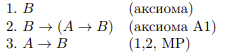
\includegraphics[width=0.35\linewidth]{images/1.1_case1.png}
    \item[(2)] Если $B \in \Gamma$, то имеем такой же вывод $A \to B$ из $\Gamma$: \newline 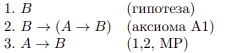
\includegraphics[width=0.35\linewidth]{images/1.1_case2.png}
    \item[(3)] Если $B = A$, то $A \to B = A \to A$. Но $\vdash A \to A$ (пример из определений \ref{a_to_a}).
    \item[(4)] Предположим теперь, что $\Gamma, A \vdash B$ и утверждение $(\,\Uparrow)$ верно для всех более коротких выводов, т.е. для всех $C$, если $\Gamma, A \vdash C$ и вывод $C$ из $\Gamma$, $A$ короче, чем вывод $B$, то $\Gamma$ $\vdash A \to C$.
    \newline Покажем, что $\Gamma \vdash A \to B$. Рассмотрим вывод из $\Gamma, A$, который заканчивается формулой $B$. При этом $B$ может оказаться аксиомой или гипотезой (тогда все предыдущие формулы для доказательства $B$ не нужны). Но в этом случае  $\Gamma \vdash A \to B$ по (1)–(3).
    \newline Остается случай, когда $B$ получается по MP из формул $C, C \to B$, причем $\Gamma, A \vdash C$ и $\Gamma, A \vdash C \to B$ с более короткими доказательствами. По предположению индукции имеем:
    \\
    \\
    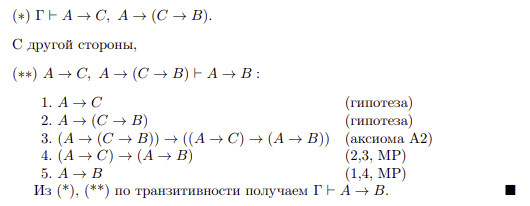
\includegraphics[width=0.8\linewidth]{images/1.1_case3.png}
\end{itemize}

\subsection{Теорема о полноте исчисления высказываний.}


\includegraphics[width=0.93\linewidth]{images/lem_1_base.png}


\includegraphics[width=0.93\linewidth]{images/lem_2_main_1.png}

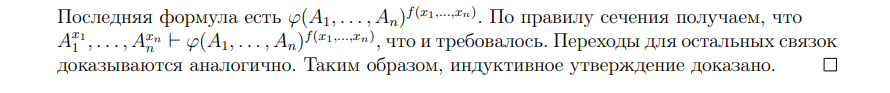
\includegraphics[width=0.93\linewidth]{images/lem_2_main_2.png}


\includegraphics[width=0.93\linewidth]{images/def_for_proof_1.png}


\includegraphics[width=0.93\linewidth]{images/th_main_for_full.png}


\includegraphics[width=0.93\linewidth]{images/proof_for_prop_1.png}


\includegraphics[width=0.93\linewidth]{images/three_lemms_for_full.png}


\includegraphics[width=0.93\linewidth]{images/the_last_lemm_full.png}

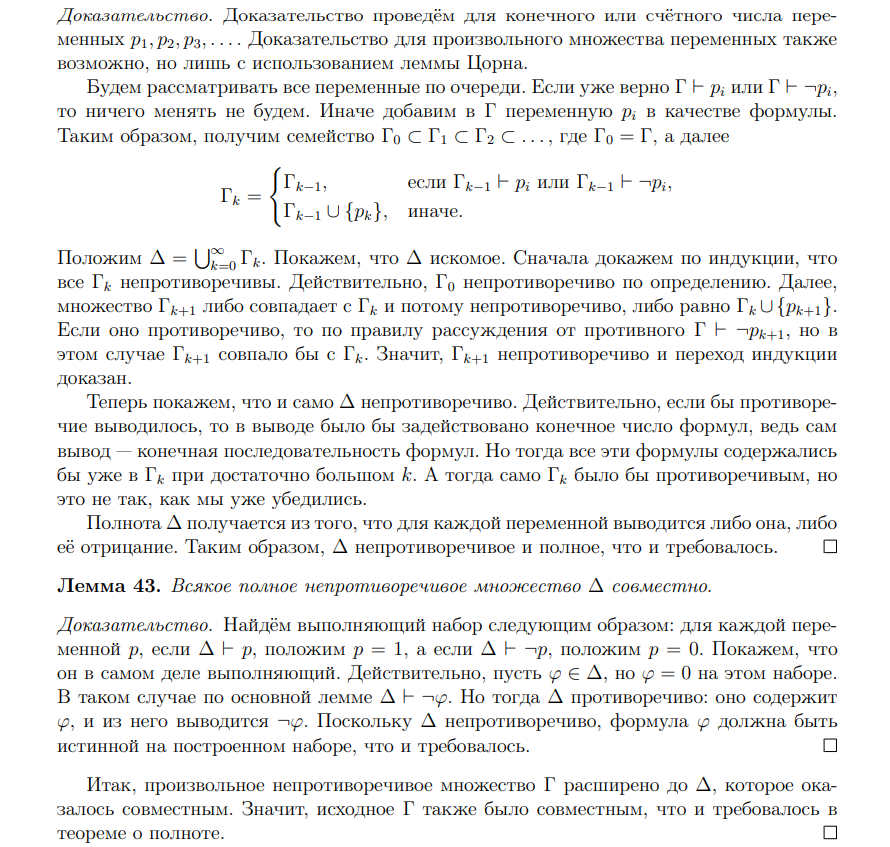
\includegraphics[width=0.93\linewidth]{images/end_of_proof_full.png}


%Из следующей теоремы нам понадобятся только 4) и 6) правила.
%\par

%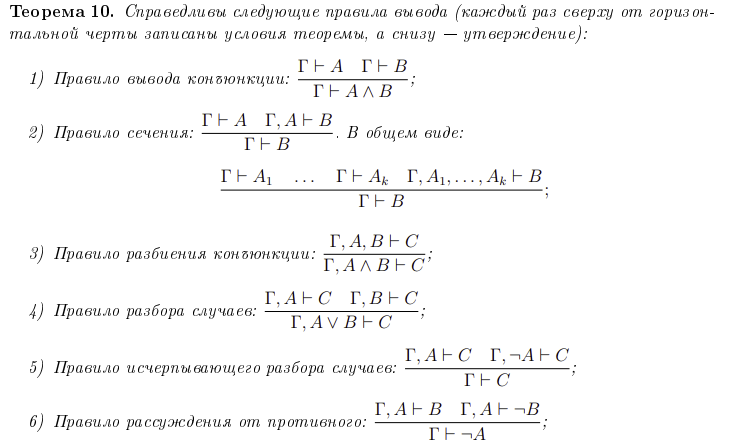
\includegraphics[width=1\linewidth]{images/1.2_theorem}

%
\includegraphics[width=0.97\linewidth]{images/1.1_v1}

%
\includegraphics[width=0.97\linewidth]{images/1.1_v3}

%
\includegraphics[width=0.97\linewidth]{images/1.1_neg}

%\par \noindent Для доказательства теоремы о полноте понадобятся две вспомогательные леммы.

%\textbf{Базовая лемма:} Представление таблицы истинности для данных четырех связок.

%\begin{tabular}{|p{1.5in}|p{1.5in}|p{1.5in}|p{1.5in}|}
%\hline
%    Для дизъюнкции: & Для конъюнкции: & Для импликации: & Для отрицания:\\ 
%    \hline
%    \centering{$A,B \vdash A\lor B$} & \centering{$A,B \vdash A \land B$} & %\centering{$A,B \vdash A\to B$} & \centering{$A \vdash \neg (\neg A)$} \tabularnewline
%    
%    \centering{$\neg A,B \vdash A\lor B$} & \centering{$\neg A,B \vdash \neg (A\land B)$} & \centering{$\neg A,B \vdash A\to B$}& \centering{$\neg A \vdash \neg A$} \tabularnewline
    
%    \centering{$A,\neg B \vdash A\lor B$} & \centering{$A, \neg B \vdash \neg (A\land B)$} & \centering{$A,\neg B \vdash \neg (A\to B)$}& \centering{} \tabularnewline
    
%    \centering{$\neg A,\neg B \vdash \neg (A\lor B)$} & \centering{$\neg A, \neg B \vdash \neg (A\land B)$} & \centering{$\neg A,\neg B \vdash A\to B$}& \centering{} \tabularnewline
%    \hline
%\end{tabular}

%\begin{enumerate}
%    \item Первые три выводимости про дизъюнкцию следуют из $A_6$ и $A_7$ по лемме о дедукции ($D$). Последняя: \newline
%    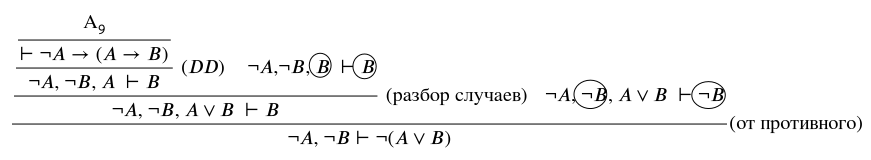
\includegraphics[width=0.99\linewidth]{images/1.1_dedu.png}
%    \item Первая выводимость про конъюнкцию следует из $A_5$ по $D$, остальные получаются контрапозицией из $A_3$ и $A_4$: \newline
%    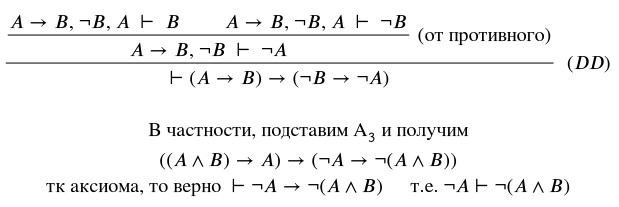
\includegraphics[width=0.8\linewidth]{images/1.1_cntrl.png}
%    \item Первая, третья и четвертая выводимость про импликацию следуют из $A_1$ и $A_9$ по $D$. Вторая выводится так: \newline
%    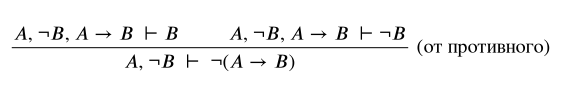
\includegraphics[width=0.7\linewidth]{images/1.1_negg.png}
%    \item Первая выводимость про отрицание доказана в утверждении 14, вторая тривиальна.
%\end{enumerate}

%\par \textbf{Основная лемма:} Пусть $\phi$ - это формула, зависящая от $p_1,\ldots,p_n$. Тогда верно следующее:
%$$p_1^{a_1},p_2^{a_2},\ldots,p_n^{a_n} \vdash \phi^{\phi(a_1,\ldots,a_n)} \text{, \qquad %где } p^a = \begin{cases}
%p, a = 1\\
%\neg p, a = 0
%\end{cases}$$
%Обозначим $a = \phi(a_1,\ldots,a_n)$

%$\blacktriangle$ Доказательство будет вестись индукцией по построению формулы с использованием базовой леммы в качестве базы и в переходе.
%\newline \textit{База индекции:} $\phi$ содержит  одну связку. Тогда это утверждение сводится к базовой лемме.
%\newline \textit{Переход:} пусть $\phi = \psi \land \gamma$. Тогда можно записать: $\phi(a_1,\ldots,a_n) = \psi(a_1,\ldots,a_n) \land \gamma(a_1,\ldots,a_n)$
%\newline Пусть $\psi(a_1,\ldots,a_n) = \alpha, \;\; \gamma(a_1,\ldots,a_n) = \beta$
%\newline Применим предположение индукции: $p_1^{a_1},\ldots,p_n^{a_n} \vdash \psi^\alpha, \;\;\; p_1^{a_1},\ldots,p_n^{a_n} \vdash \gamma^\beta$
%\newline Воспользуемся базовой леммой:
%$\psi^\alpha, \; \gamma^\beta \vdash (\psi \land \gamma)^{(\alpha\land\beta)}=\phi^a $
%\newline Записав все выводы подряд, получаем: $p_1^{a_1},p_2^{a_2},\ldots,p_n^{a_n} \vdash \phi^{a}$
%\newline Аналогичные действия проделаем и для других связок. Имеются база и переход, значит, по индукции докажем лемму для всех формул. $\qquad \blacksquare$

%\textit{Пример:} $\phi=\neg p \land (q\lor r); \quad \phi(0,1,0)=1;\quad \phi(1,0,0)=1$

%Лемма утверждает следующее: $\quad \neg p, q, \neg r \vdash \phi; \qquad p, \neg q, \neg r \vdash \neg \phi$
%\newline \par \textbf{Теорема о полноте ИВ:} Если формула $\phi$ является тавтологией, то тогда $\phi$ -- выводима. 

%$\blacktriangle$ Пусть $\phi$ -- тавтология. Тогда $\forall a_1\ldots a_n \;\; \phi(a_1,\ldots,a_n) = 1$. Значит, по основной лемме $ p_1^{a_1},p_2^{a_2},\ldots,p_n^{a_n} \vdash \phi$ при $\forall a_1\ldots a_n$. Далее воспользуемся правилом исчерпывающего разбора случаев, а также закон исключенного третьего: \newline
%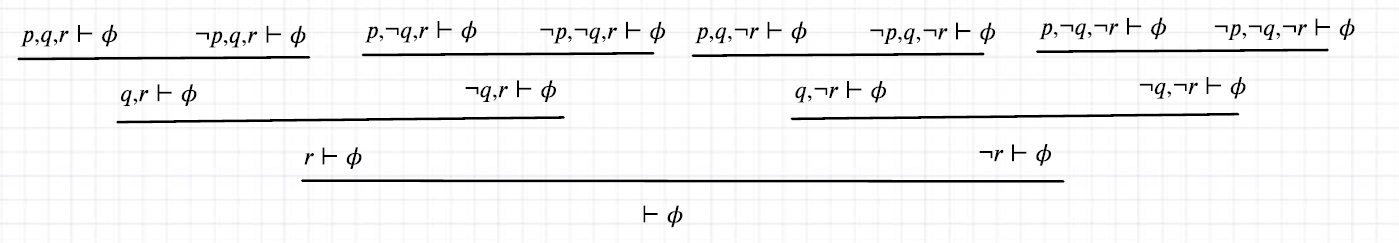
\includegraphics[width=1\linewidth]{images/1.1_cases.png}
%Такое рассуждение можно провести не только для трех литералов, но и для любого количества. Значит, теорема о полноте доказана. $\qquad \blacksquare$



\subsection{Теорема о полноте метода резолюций: из невыполнимой КНФ всегда можно вывести $\perp$.}

\textbf{Теорема.} Метод резолюций всегда заканчивает свою работу, причём для невыполнимых КНФ выводится $\perp$ (полнота), а для выполнимых не выводится (корректность).


\includegraphics[width=0.95\textwidth]{images/resolut_proof_1.png}


\includegraphics[width=0.95\textwidth]{images/resolut_proof_2.png}


\subsection{Теорема о компактности для исчисления высказываний.}

\textbf{Теорема:} Пусть любое конечное подмножество множества $\Gamma$ совместно. Тогда и всё множество $\Gamma$ совместно.

$\blacktriangle$ Если всё множество $\Gamma$ несовместно, то оно противоречиво. Но тогда в нём есть конечное противоречивое подмножество. Но тогда оно несовместно, что противоречит условию. $\quad \blacksquare$

\subsection{Устойчивость выразимых предикатов при автоморфизмах интерпретаций.}

Пусть имеется некоторая сигнатура $\sigma$ и интерпретация этой сигнатуры, носителем которой является множество $M$.

\textbf{Определение:} Взаимно однозначное отображение $\alpha: M \to M$ называется \textit{автоморфизмом} интерпретации, если все функции и предикаты, входящие в интерпретацию, устойчивы относительно $\alpha$. При этом k-местный предикат $P$ называется \textit{устойчивым} относительно $\alpha$, если 
\[P(\alpha(m_1), \ldots, \alpha(m_k)) \lra P(m_{1}, \ldots, m_{k})\]
для любых элементов $m_1, \ldots, m_k \in M$. Далее, k-местная функция $f$ называется устойчивой относительно $\alpha$, если
\[f(\alpha(m_{1}), \ldots, \alpha(m_{k})) = \alpha(f(m_{1}, \ldots, m_{k})).\]

\textbf{Теорема:} Любой предикат, выразимый в данной интерпретации, устойчив относительно её автоморфизмов.

$\blacktriangle$ Пусть $\pi$ — некоторая оценка, то есть отображение, ставящее в соответствие всем индивидным переменным некоторые элементы носителя. Через $\alpha \circ \pi$ обозначим оценку, которая получится, если к значению каждой переменной применить отображение $\alpha$; другими словами, $\alpha \circ \pi (\xi) = \alpha(\pi(\xi))$ для любой переменной $\xi$.

Первый шаг состоит в том, чтобы индукцией по построению терма t доказать такое утверждение: значение терма t при оценке $\alpha \circ \pi$ получается применением $\alpha$ к значению терма t при оценке $\pi$: $[t](\alpha \circ \pi) = \alpha([t](\pi))$.

Для переменных это очевидно, а шаг индукции использует устойчивость всех функций интерпретации относительно $\alpha$. Теперь индукцией по построению формулы $\varphi$ легко доказать такое утверждение: $[\varphi](\alpha \circ \pi) = [\varphi](\pi)$.

Мы не будем выписывать эту проверку; скажем лишь, что взаимная однозначность $\alpha$ используется, когда мы разбираем случай кванторов. (В самом деле, если с одной стороны изоморфизма берётся какой-то объект, то взаимная однозначность позволяет взять соответствующий ему объект с другой стороны изоморфизма.)
$\blacksquare$

\subsection{Теорема Гёделя о полноте исчисления предикатов: расширение любого непротиворечивого множества до полного и экзистенциально полного.}

\textbf{Определение:} Множество Г замкнутых формул в сигнатуре называется теорией.

\textbf{Определение:} Интерпретация $M$ сигнатуры $\sigma$ называется моделью теории Г, если все формулы из Г истинны в $M$.

\textbf{Определение:} Теория Г называется совместной, если все формулы из Г могут быть одновременно истинны в некоторой интерпретации.

\textbf{Определение:} Теория Г называется противоречивой, если из нее выводится некоторая формула $\phi$ и ее отрицание $\neg\phi$, и непротиворечивой в противном случае.

\par
\textbf{Теорема Гёделя о полноте исчисления предикатов}:
Если $\varphi$ общезначима, то она выводима в исчислении предикатов.
Пользуясь данной терминологией, можно сформулировать теорему, из которой будет следовать теорема Гёделя.

\textbf{Теорема}: Если теория непротиворечива, то она совместна (имеет модель).

\textbf{Доказательство:} 1. Мы хотим расширить не противоречивую Г так, чтобы она была полной (если $\varphi$ - замкнутая формула, то Г $ \vdash \varphi$ или  Г $ \vdash \neg \varphi$) и экзистенциально полной (т.е. если Г $ \vdash \exists x \varphi$, то Г $ \vdash \varphi(t/x)$, где t - замкнутый терм.
\begin{center}
    
\includegraphics[width=13cm]{images/1.5_m1}

    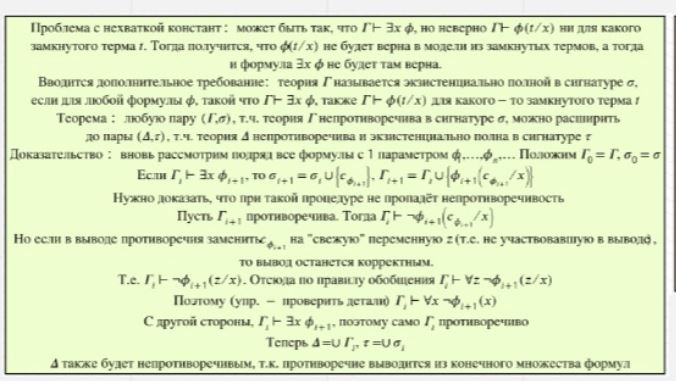
\includegraphics[width=13cm]{images/1.5_m2}

    
\includegraphics[width=12cm]{images/1.5_m3}

    
\includegraphics[width=12cm]{images/1.5_full}
\end{center}

\textbf{Лемма 9}.
Любую непротиворечивую теорию можно расширить до непротиворечивой, полной и экзистенциально полной теории.

Доказательство было приведено выше.

\subsection{Теорема Гёделя о полноте исчисления предикатов: построение модели из замкнутых термов у любого непротиворечивого, полного и экзистенциально полного множества.}

\textbf{Лемма 10}.

Любая непротиворечивая, полная, экзистенциально полная теория совместна, то есть имеет модель.
\begin{center}
    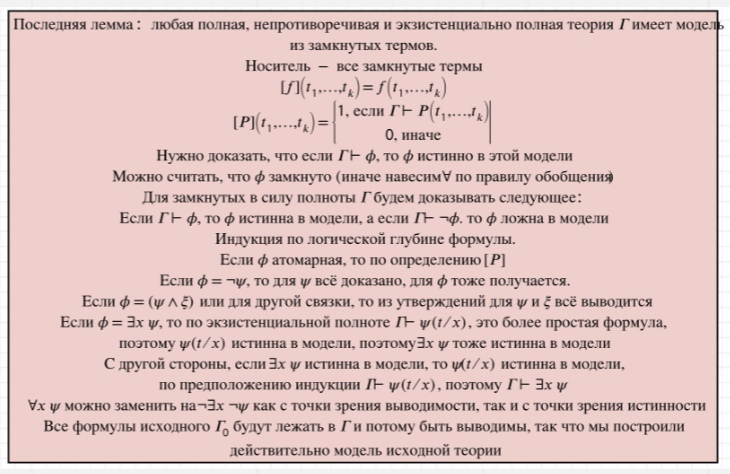
\includegraphics[width=12cm]{images/1.5_full2}    
\end{center}

\subsection{Представимость конечных последовательностей в арифметике при помощи $\beta$-функции Гёделя.}

\textbf{Лемма 1}:\\

$\forall n \quad \forall c \quad \exists b > c$ такое, что $b + 1,  2b + 1, \dotsc, nb + 1$ - взаимно просты.\\

Рассмотрим $b = n!$.

Тогда возьмем произвольные различные $k$ и $m$ от $1$ до $n$. $gcd(kb + 1, mb + 1) = d > 1 \Rightarrow (k - m)b$ делится на $d$.

Значит т.к. $b = n!$ и $k - m < n$, получаем, что любой простой делитель числа $(k - m)b$ должен быть строго меньше $n$.\\

У $d$ есть простой делитель $p < n$.

$mb + 1$ делится на $p$.

$mb + 1 - m\cdot n!$ делится на $p \Rightarrow d = 1$ 
\\

\textbf{Лемма 2.}\\

$\forall (x_1, \dotsc, x_n) \quad\exists a, b \quad \forall i : a \equiv x_i \quad mod (b_i + 1)$\\

\textbf{Док-во:}\\

Выберем по Лемме 1 $b > max\{x_i\}$.\\

Тогда нужное $a$ найдётся по китайской теореме об остатках: Если натуральные числа $a_1, \dotsc, a_n$  попарно взаимно просты, то для любых $r_1, \dotsc, r_n$ таких, что $0 \leq r_i < a_i$ при всех $i : 0, \dotsc, n$ найдется число, которое при делении на $a_i$ дает остаток $r_i$ при всех $i$. Более того, если найдутся два таких числа, то они будут сравнимы по модулю $a_1 \cdot \dotsc \cdot a_n$.\\

Положим $\beta(a, b, i) = a \quad mod (bi + 1)$

$\beta$ арифметична: $r = x \quad mod(q) \Leftrightarrow r < q$ и $\exists s: x = sq + r$.

\subsection{Арифметичность предикатов «n — степень шестёрки» и $n = 2^k$.}

\textbf{Определение:} Предикат $P: \N^k \to \{0,1\}$ называется \textit{арифметичным}, если он выразим в стандартной интерпретации арифметики $\langle \N, +, \cdot, = \rangle$. Функция $f: \mathbb{N}^k \rightarrow \mathbb{N}$ называется \textit{арифметичной}, если арифметичен предикат $P_{f}: \mathbb{N}^{k+1} \rightarrow \{0,1\}$, где $P_f(x,y) = 1 \lra f(x) = y$.
\\
\\
\textbf{Степень шестерки}
\\
Степень шестерки можно выразить с использованием квантора по конечному множеству\\
    $\exists D (x \in D \wedge \forall y \in D (y = 1 \vee (y \ \vdots \ 6 \wedge \frac{y}{6} \in D)))$ \\ У нас есть $x, \frac{x}{6}, \frac{x}{36}, \frac{x}{216}, ..., 1$. Этакий мешок с числами. И если в нем есть х, то есть и $\frac{x}{6}$ и т.д., а остановиться это все может только на единице. Соответственно, если x - не степень шестерки, то возникнет не единица, и оба условия будут нарушены.
    \\
    \\
    Через обычные предикаты эта функция выражается с помощью кодирования Смаллиана. Оно лучше применимо для описания конечных множеств. В чем суть:
    \\
    Берем и вводим предикат $S(a,b,x)$, которые отвечает следующим свойствам:
    \begin{itemize}
        \item [1] $\forall a,b\{x: S(a,b,x) = 1\}$ - конечно
        \item[2] Для любого конечного S найдутся такие a и b, что $S = \{x: S(a,b,x) = 1\}$
    \end{itemize}
    Теперь записанную нами формулу $\exists D .... x \in D....$ можно переписать следующим образом:\\
    $\exists a,\exists b (S(a,b,x) \wedge \forall y(S(a,b,y) \rightarrow (y = 1 \vee(y \ \vdots \ 6 \wedge \exists z(y = 6\cdot z \wedge S(a,b,z))))))$ \\
    Что поменялось? Заменили $\exists D$ на $\exists a, \exists b$. И $x \in D$ на $S(a,b,x)$, получили формулу первого порядка\\\\
\textbf{Степень двойки}\\
$x = 2^k $ можно выразить с использованием квантора по конечной последовательности\\
$\exists \{a_i\} (a_0 = 1 \wedge a_k = x \wedge \forall i \in [0;k-1] \ a_{i+1} = a\cdot a_i)$
\\
\\
Через обычные предикаты это выражается с использованием $\beta$-функции Гёделя. 
\\
Тут вводится арифметическая функция $\beta(a,b,i)$ со следующим свойством:
\begin{itemize}
    \item[] $\forall [x_0, ..., x_n]$ найдутся такие a,b, что $\forall i \in [0,n] \ x_i = \beta(a,b,i)$
\end{itemize}
Теперь в формуле, которая имеет вид $\exists \{x_i\} ......x_j......$ можно заменить на такую: $\exists a \exists b ......\beta(a,b,j)......$
\\
\\
Применим полученные знания к нашему предикату и получим:\\
$x = 2^k \Longleftrightarrow \exists a,b \ (\beta(a,b,0) = 1 \wedge \beta(a,b,k) = x \wedge \forall i \in [0,..., k-1] \ \beta(a,b,i+1) = 2\cdot \beta(a,b,i) $


\subsection{Множество замкнутых формул, истинных в $\mathbb N$, неперечислимо. Первая теорема Гёделя о неполноте.}

\textbf{Опр} Множество A $\subset \mathbb{N}^k$ называется \textit{арифметическим}, если существует арифметическая формула $\alpha$ с параметрами $x_1, . . . , x_k$, которая его представляет в следующем смысле: $<n_1, . . . , n_k>$ принадлежит множеству A тогда и только тогда, когда формула $\alpha$ истинна при значениях параметров $x_1 = n_1, . . . , x_k = n_k$.
\\
\\
Любое перечислимое множество арифметично
\\
\\
\textbf{Лемма1}\\
Всякое арифметическое множество лежит в классе $\Sigma_n$ или $\Pi_n$ для некоторого n (и, естественно, для всех больших n).
\\
$\blacktriangle$ Формулу, задающую арифметическое множество, приведём к предварённой нормальной форме (вынеся кванторы наружу). Ясно, что бескванторная часть задаёт разрешимое множество, поэтому исходное множество принадлежит какому-то из классов $\Sigma_n$ или $\Pi_n$. Можно и не использовать предварённой нормальной формы, а применить индукцию по длине формулы и сослаться на то, что пересечение, объединение и дополнение, а также проекция не выводят за пределы арифметической иерархии (объединения всех классов $\Sigma_n$ и $\Pi_n$). $\blacksquare$
\\
\\
Рассмотрим теперь множество T, элементами которого являются
все истинные арифметические формулы без параметров (точнее, их номера в какой-то вычислимой нумерации всех формул — это значит, что по формуле можно алгоритмически получить её номер и наоборот).
\\
\\
\textbf{Лемма2}\\ Любое арифметическое множество m-сводится к множеству T.\\
$\blacktriangle$ Пусть A — произвольное арифметическое множество. Пусть $\alpha$(x) — формула с одной переменной, которая выражает принадлежность множеству A. Это означает, что $\alpha$(n) истинно при тех и только тех n, которые принадлежат A.
Тогда вычислимая функция n $\rightarrow$ (номер формулы, которая является
результатом подстановки константы n в $\alpha$(x)) m-сводит A к T. $\blacksquare$
\\
\\
\textbf{ Первая теорема
Гёделя о неполноте}\\
Множество T арифметических истин неперечислимо.\\
$\blacktriangle$ Это следует из того, что если бы Т было перечислимо, оно было бы арифметично, что противоречит теореме Тарского $\blacksquare$ 
\\
\\
\textbf{Множество замкнутых формул, истинных в N, неперечислимо } \\
Если множество перечислимо, то оно лежит в арифметической иерархии, что противоречит теореме Тарского


\subsection{Теорема Тарского.}

\textbf{Теорема Тарского}\\
Истинность арифметической формулы нельзя выразить арифметическим выражением. То есть не существует формулы True(x), которая истинна тогда и только тогда, когда формула с номером х истинна. (Множество T не арифметично.)
\\
$\blacktriangle$ Если бы T было арифметическим, то оно лежало бы в некотором конкретном классе . Поскольку всякое арифметическое множество сводится к T, то все арифметические множества лежали бы в этом классе. Но мы знаем, что множества из более высоких классов иерархии тоже арифметичны, но в $\Sigma_n$ не лежат.$\blacksquare$

    \newpage
    \section{№2 Не абелевы группы}

\begin{reminder}
    Группа $(G, \cdot)$
    \begin{itemize}
        \item $(G1): x \cdot (y \cdot z) = (x \cdot y) \cdot z$ 
        \item $(G2): \exists c \in G \  \forall x: \ x \cdot e = e \cdot x = x$ 
        \item $(G3): \forall x \in G \  \exists x^{-1}: \ x \cdot x^{-1} = x^{-1} \cdot x = e$ 
        \item Абелевы группы: $x \cdot y = y \cdot x$
        \end{itemize}

\end{reminder}

\subsection{Группы биекций}

\begin{itemize}
    \item Тотальная функция: $f: A \ra B$
    \item Инъекция $\Lra f(x_1) = f(x_2) \Ra x_1 = x_2$
    \item Сюръекций $\Lra \forall y \in B \  \exists x \in A: \ f(x) = y$
    \item Биекция $\Lra$ инъекция и сюръекция
\end{itemize}

\subsection{Композиция функций}

\begin{definition}
    Пусть заданы функции $f, g: A \ra A$. Тогда их композицией будет:

    $(f \circ g)(x) = f(g(x))$
\end{definition}


\begin{example}
    $(S(x), +)$ --- группа.

    Где, $X$ --- множество, $S(x)$ --- биекция $X \ra X$.
\end{example}


% Пример: $(S(x),\  +)$ -- группа \\
% X -- множество \\
% S(x) -- биекция $X \rightarrow X$ \\


% Композиция \\
\begin{note}
    \[\big( (f \comp g) \comp h \big)(x) = \big( f \comp (g \comp h) \big)(x) \Ra\]
    \[\Ra \bigl( \big(g(h(x))\big) \bigl)\]
    \[\id : \ x \raone x\]
\end{note}

% $id: x \rightarrow x$ \\

Обратная функция --- просто биекция в другую сторону

\begin{example}[Не абелевой группы]
    \[f: \  x \raone x + 1\]
    \[g: \  x \raone -x\]
    \[(f \comp g)(x) = -x + 1\]
    \[(g \comp f)(x) = -x - 1\]
    Т.е. порядок имеет значение.
\end{example}
% Пример: \\
% $f: x \rightarrow x + 1$ \\
% $g: x \rightarrow -x$ \\
% \[(f \circ g)(x) = -x + 1\] 
% \[(g \circ f)(x) = -x - 1\], т.е. не равны \\

\newpage
\subsection{Перестановки}

\begin{definition}
    $X = \left \{1, 2, \dots n \right \}$ --- множество $n$ элементов.

    $S_n = S(x)$ --- группа перестановок степени $n$.
\end{definition}

\begin{enumerate}
    \item[I.] \ul{Размещение} из $n$ по $n$. 
    
    34512
    \item[II.] \ul{Табличный}
    
    \[
        \Pi = 
        \begin{pmatrix}
            1 2 3 4 5 \\
            3 4 5 1 2
        \end{pmatrix}
        \]
        
        $\Pi (1) = 3$.
        
        \[
        \sigma = 
        \begin{pmatrix}
            1 2 3 4 5 \\
            2 1 3 4 5
        \end{pmatrix}
        \]
        
        \[
        (\Pi \  \circ \  \sigma)  = 
        \begin{pmatrix}
            1 2 3 4 5 \\
            $\st{21345}$ \\
            4 3 5 1 2
        \end{pmatrix}
        \]
    \item[III.] \ul{С помощью графа}. Входящие и исходящие степени равны по 1, так как является биекцией.

    \[\Pi = (13524) = (52413)\]
    \[\sigma = (12)\] Bключая циклы длины 1 (просто их не пишем).
    
    \[(\Pi \circ \sigma) = (14)(23)\]
    
\end{enumerate}

% 1. Размещение из n по n \\
% $2451$ \\

% 2. Табличный \\
% \[
% \Pi = 
% \begin{pmatrix}
%     1 2 3 4 5 \\
%     3 4 5 1 2
% \end{pmatrix}
% \]

% $\Pi (1) = 3$

% \[
% \sigma = 
% \begin{pmatrix}
%     1 2 3 4 5 \\
%     2 1 3 4 5
% \end{pmatrix}
% \]

% \[
% (\Pi \  \circ \  \sigma)  = 
% \begin{pmatrix}
%     1 2 3 4 5 \\
%     2 1 3 4 5 \\
%     4 3 5 1 2
% \end{pmatrix}
% \], и вычеркнем центральную линию.

% 3. С помощью графа. Входящие и исходящие степени равны по 1, т.к. является биекцией.
% \[\Pi = (13524) = (52413)\]
% \[\sigma = (12), \] исключая циклы длины 1 (просто их не пишем).

% \[(\Pi \circ \sigma) = (14)(23)\]

% \subsection{Продолжение не абелевых групп}

\subsection{Общие свойства групповых операций}

\begin{enumerate}
    \item \ul{Закон сокращения}:
    \[\forall a \in G: \  x = y \Leftrightarrow ax = ay \Leftrightarrow xa = ya\]
    \[a^{-1}(ax) = (a^{-1}a)x = ex = x\]

    \item \ul{Формула обратного произведения}:
    \[(xy)^{-1} = y ^ {-1} \cdot x ^{-1}\]
    \[(xy)(y^{-1}x^{-1}) = x(y y^{-1}) x^ {-1} = xex^{-1} = x x^{-1} = e\]
    Проверка, что обратный единственный: \\
    \[C = x u = xv\] и получаем желаемое.
\end{enumerate}

% 1. Закон сокращения: \\
% \[\forall a \in G \  x = y \Leftrightarrow ax = ay \Leftrightarrow xa = ya\]
% \[a^{-1}(ax) = (a^{-1}a)x = ex = x\]

% 2. Формула обратного произведения: \\
% \[(xy)^{-1} = y ^ {-1} \cdot x ^{-1}\]
% \[(xy)(y^{-1}x^{-1}) = x(y y^{-1}) x^ {-1} = xex^{-1} = x x^{-1} = e\]
% Проверка, что обратный единственный: \\
% \[C = x u = xv,\] и получаем желаемое.

\subsection{Подгруппы}

\begin{definition}
    Подгруппа $H$ группы $G$: $H \subseteq G$ ($H < G$) (групповая операция та же самая).
\end{definition}

\begin{example}
    $3 \mathbb{Z}  = \left\{ x \mid x = 3y,\  y \in \mathbb{Z} \right\}$
\end{example}

\begin{definition}
    $GL(\mathbb{R}, n)$ --- общая группа линейных преобразований.
\end{definition}


Проверка, что элементы принадлежит группе:
\begin{itemize}
    \item[\text{$\left. 1 \right)$}] $e_G \in H: \begin{cases} e_H \cdot h = h, \\ e_G \cdot h = h \end{cases} \Ra e_H = e_G$
    \item[\text{$\left. 2 \right)$}] $x \in H \Ra x ^ {-1} \in H: \begin{cases} x_H^{-1} x = e, \\ x_G^{-1} x = e \end{cases} \Ra x_H^{-1} = x_G^{-1}$
    \item[\text{$\left. 3 \right)$}] $x, y \in H, \  x \cdot y \in H$
\end{itemize}

\begin{reminder}
    Вычеты --- $\bar{n} \ZZ \quad \left[a \right]_n = \left\{ x: x = a + z, z \in \bar n \ZZ \right\}$ ($H < G, \ g \in G$)
\end{reminder}

\begin{definition}
    ~

    Смежный (левый) класс --- $gH = \left\{x \mid x = gh, h \in H\right\}$,
    
    Смежынй (правый) класс --- $Hg = \left\{x \mid x = hg, h \in H\right\}$
\end{definition}

\begin{lemma}
    Смежные классы не пересекаются или совпадают.
\end{lemma}
\begin{proof}
    \begin{gather}
        z \in xH \  \land \  yH \quad z = x h_1 = y h_2, \quad h_1, h_2 \in H \\
        \begin{cases} x = y(h_2h_1^{-1}) \in yH, \quad xH \subseteq yH, \\
        xh_1 = y (h_2h_1^{-1}h_1) \in yH, \quad yH \subseteq xH \end{cases} \Ra xH = yH
    \end{gather}
\end{proof}

\subsection{Порядок группы}

\begin{definition}
    $|H| < \infty$ --- порядок группы.
\end{definition}

\[\Rightarrow |gH| = |H|\]
\[\alpha: H \ra gH\]
\[\alpha(h) = gH\]

\[gh_1 = gh_2 \Rightarrow h_1 = h_2\]

\begin{definition}
    $(G: H)$ --- индекс подгруппы (число смежных классов).
\end{definition}

\begin{theorem}[Лагранж]
    $|G| = |H| \cdot (G: H)$
\end{theorem}

\begin{itemize}
    \item[$1^{0}$] Порядок подгруппы делит порядок группы.
    \item[$2^{0}$] $|G| = p$ --- простое. В $G$ нет совместных подгрупп $\left\{ e \right\}, G$ --- несобственные.
    \item[$3^{0}$] $|G| = p$ --- простое, то $G$ -- абелева.
\end{itemize}

\begin{definition}
    $\langle g \rangle$ --- наименьшая подгруппа, содержащая g.
\end{definition}

\[\langle g \rangle = \left\{ e = g^0, g^1, g^2, \dots, g^{-1}, g^{-2} \right\}\]
\[\forall g: \ \langle g \rangle < G, \ |G| = p \Rightarrow \langle g \rangle = G\]

\begin{definition}
    Порядок элементов в группе --- $\ord g = |\langle g \rangle| \Leftrightarrow $ наименьшее $k: \  g^k = e$

\end{definition}

\begin{example}
    Рассмотрим группу: $(\ZZ_n, +)$
    \[\langle a \rangle = {\left [ ka \right ]}_n\]
    \[\ord a = \min k: ka \equiv 0 \mod n = \frac{\lcm (a, n)}{a} = \frac{n}{\gcdru (a, n)} \Ra\]
    \[\Ra \gcdru (a, n) \cdot \lcm (a, n) = a \cdot n\]
\end{example}


% $\langle a \rangle = {\left [ ka \right ]}_n$

% $\ord a = \min l: ka \equiv 0 \mod n = \frac{\lcm (a, n)}{a}$

$|\langle d \rangle| = \frac{n}{d}$

$|(\ZZ^{\text{*}}_n, \cdot)| = \phi (n) $ --- функция Эйлера.

\begin{theorem}[\text{Эйлер}]
    \[\gcdru(a, n) = 1 \Ra a^{\phi (n)} \equiv 1 \mod n\]
    \[k \cdot \ord a = \phi(n)\]
    \[a ^ {k \ord a} = (a ^ {\ord a})^k = 1 ^ k = 1\]
\end{theorem}

\begin{theorem}[\text{Малая теорема Ферма}]
    Если $p$ --- простое, то:
    \[a \not \equiv 0 \mod p \Ra a^{p - 1} \equiv 1 \mod p\]
\end{theorem}


    \newpage
    \section{№3 Изоморфизм группы}

\begin{reminder}
  наименьшее k --- порядок группы, если $g ^ k = e$.
\end{reminder}

\begin{note}
  $(Z_n, +) \quad \ord a = \frac{n}{\gcdru(a, n)}$
  \[S_n \ord \Pi = \gcdru(\text{\#len}).\] Где \#len --- длинна циклов.
\end{note}

\subsection{Порядки перестановки}

\begin{reminder}
  $\Pi: (a_0, a_1, \dots, a_{l - 1})$. Если $\Pi ^ {s} = \id \Ra \Pi ^{s} (a_0) = a_0 \Ra l \mid s$
  \[\ord \Pi = l.\]
\end{reminder}

\begin{example}
  $\pi = \underbrace{(\dots)}_{l_1}\underbrace{(\dots)}_{l_2}\underbrace{(\dots)}_{l_3} \dots \underbrace{(\dots)}_{l_s}$. Тогда имеем $\ord \pi = \gcdru(l_1, \dots, l_s).$
\end{example}

\begin{example}
  $\mid G \mid = n, \ d = 80, \ \mid S_{12} \mid = 12!$
  \[\gcdru(l_1, \dots, l_s) = 80, \]
  \[l_1 + \dots + l_s = 12.\]
  То есть невозможно.
\end{example}

\subsection{Основная теорема арифметики}
\begin{theorem}[Основная теорема арифметики]
  Для любого n > 1 --- \ul{однозачно} представялется произведением простых множителей (с точностью до пересестановки множителей).
\end{theorem}

\begin{example}
  $80 = 2 ^ 4 \cdot 5 = 2 ^ 2 \cdot 5 \cdot 2 ^ 2$.
\end{example}

\begin{proof}
  По индукции. $n = 2$ --- база. Пусть < n --- существует.
  \begin{enumerate}
    \item[(1)] n --- простое,
    \item[(2)] $n = ab, \ 1 < a, b < n$.
  \end{enumerate}
  Пусть $x \not \equiv 0 \mod p \Ra x^{-1} \cdot x \equiv 1 \mod p \Ra y \equiv 0 \mod (p)$.
\end{proof}

\begin{lemma}
  p --- простое, то есть $xy \equiv 0 \mod (p) \Ra$
  \[x \equiv 0 \mod (p) \vee y \equiv 0 \mod (p).\]
\end{lemma}

\begin{proof}
  $\underbrace{p_1 \dots p_k}_{\text{Делится на } p_1} = q_1 \dots q_s$, где $p_i, q_j$ --- простое. Тогда утверждается, что $p_i \not = q_i$ --- в силу закона сокращения.
  \[\Ra p_1 \mid q_k \Ra p_1 = q_k.\] В силу того, что левая часть делится на $p_1$.
\end{proof}

\begin{proposition}
  $n = p_1^{a_1} \dots p_t^{a_t} \dots, \quad p_1 < p_2 < p_3 < \dots < p_t < \dots$
  \[p_k \nmid n \Ra a_k = 0.\]
\end{proposition}

\begin{example}
  \[x = p_1^{a_1} \dots p_t^{a_t} \dots ,\]
  \[y = p_1^{b_1} \dots p_t^{b_t} \dots ,\]
  \[x \mid y \Lra a_i \leq b_i,\]
  \[\gcdru(x, y) = p_1^{\min (a_1, b_1)} \cdot \ldots \cdot p_t^{\min (a_t, b_t) },\]
  \[\lcm(x, y) = p_1^{\max (a_1, b_1)} \cdot \ldots \cdot p_t^{\max (a_t, b_t) }.\]
\end{example}

\subsection{Класс групп}
\begin{definition}
  Группа G --- циклическая, если:
  \[G = \langle g \rangle.\]
  Обозначение: $C_n$ --- циклическая.
\end{definition}

\begin{corollary}
  Любая циклическая группа --- абелева. То есть, для любого элемента выполнено: $g^{i + j} = g^i \cdot g^j$.
\end{corollary}

\begin{example}
  $| (Z_{\delta}^{\text{*}}, \cdot) | = 4, \quad 1^2 \equiv 3^2 \equiv 5^2 \equiv 7^2 \equiv 1 \mod \delta$.
\end{example}

\begin{theorem}
  Если, $G = \{ g^i, i \in \ZZ \} = \langle g \rangle$, то изоморфны и $(\ZZ, +)$ и $(Z_n, +)$.
\end{theorem}

\begin{example}
  $|G| = \infty$ --- все степени различны.
  \[g^i = g ^ j \Lra g^{j - i} = e,\]
  \[k \raone g^k,\]
  \[(\ZZ, +) \ra G,\]
  \[g^{n + qn} = g^i \cdot g^{qn} = g^i \cdot (g^n)^q.\]
\end{example}

\begin{theorem}
  Подгруппа циклической группы --- циклическая.
\end{theorem}

\begin{example}
  Пусть $G < (\ZZ, +)$, тогда 
  \[\quad d = \min (x: x > 0 \quad x \in G), \]
  \[g \in G \quad g = qd + r, \ 0 \leq d, \]
  \[t = g - qd \in G \Ra r = 0.\]
  Если $G < (Z_n, +)$, тогда
  \[d  = \min (x: 0 < x < n \quad [x] \in G),\]
  \[d \mid n \quad n = qd + r \Ra r \in G \Ra r = 0.\]
\end{example}

\subsection{Изоморфизм групп}
\begin{example}[1]
  $(Z_6, +)$. Нейтальный --- $0$. Кратные элементы --- $ka$.
\end{example}

\begin{example}[2]
  $g = \langle(12)(345)\rangle, \quad \ord g = 6$
\end{example}

\begin{definition}
  Изоморфизм групп, это отображение, такое что:
  \[\phi : G_1 \ra G_2\]
  \begin{enumerate}
    \item[(1)] $\phi$ --- биекция,
    \item[(2)] $\phi(xy) = \phi(x) \ \phi(y)$. Для любых $x, y \in G$.
  \end{enumerate}
  Обозначение: $G_1 \cong G_2$.
\end{definition}

\begin{note}
  Тогда имеем, что примеры (1) и (2) --- изоморфны.  
\end{note}

\subsection{Прямое произведение групп}
\begin{definition}
  Пусть G, H --- группы. Тогда, $G \times H = \{(g, h): g \in G, h \in H\}$. Тогда имеем несколько свойств: 
  
  \begin{enumerate}
    \item $(g_1, h_1) \cdot (g_2, h_2) = (g_1 \cdot g_2, h_1 \cdot h_2)$,
    \item $\ord (g, h) = \lcm(\ord g, \ord h)$,
    \item $(g, h)^k = (g^k, h^k) = (e, e)$.
  \end{enumerate}
\end{definition}

\begin{proposition}
  $\gcdru(p, q ) = 1$, тогда имеем: $C_p \times C_q \cong C_{pq}$.
\end{proposition}

\begin{proof}
  $\ord(1, 1) = \gcdru(p, q) = \frac{pq}{1} = pq = |C_p \times C_q|$.
\end{proof}

\begin{corollary}
  $C_p \times C_q \text{--- циклическая} \cong C_{pq}$.
\end{corollary}

\subsection{Мультипликативность функции Эйлера}

\begin{proposition}
  % $\gcdru(p, q) = 1 \Ra \underbrace{\phi(pq)}_{\text{Число порождающих в } C_{pq}} = \underbrace{\phi(p) \phi (q)}_{\text{Число порождающих в } C_p \times C_q}$
  Если $\gcdru(p, q) = 1$, то выполено равенство:
  \[\phi(pq) = \phi(p) \phi (q).\]

  % $\phi(n) = |(Z_n^{\text{*}}, \cdot)|$
\end{proposition}

\begin{proof}
  Равенство верное, в силу того, что левая часть --- число порождающих в $C_{pq}$, а справа --- число порождающих в $C_p \times C_q$.
\end{proof}

\begin{proposition}
  Количество пораждающих в $C_n$ равно $\phi(n)$.
\end{proposition}

\begin{proof}
  \[(x, y) \in C_p \times C_q, \]
  \[\ord (x, y) = \gcdru(\ord x, \ord y) = pq \Ra \ord x = p, \quad \ord y = q.\]    
\end{proof}

\begin{example}
  Пусть $n = p_1^{q_1} \dots p_t^{a_t}, \quad a_i > 0$, тогда

  \[\phi (p^n) = p^n - p^{n - 1}.\]В силу того, что $x \not \equiv 0 \mod (p^n) \Lra x \equiv 0 \mod (p)$.

  \[\phi(n) = (p_t^{a_t} - p_t^{a_t - 1}) = n (1 - \frac{1}{p_1}) (1 - \frac{1}{p_2}) \dots (1 - \frac{1}{p_t}).\]
\end{example}



    \newpage
    \section{4. Степенные ряды. Теорема Коши-Адамара. Радиус и круг сходимости, равномерная сходимость степенных рядов. Теорема Абеля. Дифференцируемость суммы степенного ряда. Теорема единственности, ряд Тейлора. Пример бесконечно дифференцируемой функции, не разлагающейся в степенной ряд. Достаточное условие разложимости функции в степенной ряд. Ряды Тейлора $e^{x}$, $\sin x$, $\cos x$, $(1 + x)^{\alpha}$, $\ln(1 + x)$.}

\begin{definition}
    \emph{Степенным рядом} называется функциональный ряд вида
    \begin{equation}
        \label{power-series}
        \sum_{n = 0}^\infty a_n (x - x_0)^n,
    \end{equation}
    где $a_n, x_0 \in \R$ и $x$ --- действительная переменная, или $a_n, x_0 \in \mathbb{C}$ и $x$ --- комплексная переменная \emph{(комплексный степенной ряд)}.
\end{definition}


\begin{theorem}[Коши-Адамар]
    \label{cauchy-hadamard}
    Пусть $R = \frac{1}{\overline{\lim}_{n \rightarrow \infty} \sqrt[n]{|a_n|}}$.

    Тогда:
    \begin{enumerate}
        \item при $|x - x_0| < R$ ряд (\ref{power-series}) сходится, причём абсолютно;
        \item при $|x - x_0| > R$ ряд (\ref{power-series}) расходится;
        \item если $r \in (0, R)$, то ряд (\ref{power-series}) равномерно сходится на $\overline{B_r}(x_0) = \{x: |x - x_0| \le r\}$.
    \end{enumerate}

    \begin{proof}
        Пусть $x \neq x_0$, тогда
        \[
            q \coloneqq \overline{\lim_{n \rightarrow \infty}} \sqrt[n]{|a_n (x - x_0)^n|} = |x - x_0| \overline{\lim_{n \rightarrow \infty}} \sqrt[n]{|a_n|} = \frac{|x - x_0|}{R}.
        \]

        Если $|x - x_0| < R$, то $q < 1$ и, значит, по признаку Коши $\sum_{n = 0}^\infty |a_n (x - x_0)^n|$ сходится, то есть, ряд (\ref{power-series}) сходится абсолютно.

        Если $|x - x_0| > R$, то $q > 1$ и, значит, по признаку Коши $n$-й член ряда не стремится к нулю, ряд (\ref{power-series}) расходится и \emph{абсолютно расходится} (то есть, расходится ряд из модулей членов).

        Пусть $r \in (0, R)$. По доказанному ряд (\ref{power-series}) абсолютно сходится в точке $x = x_0 + r$, то есть сходится ряд $\sum_{n = 0}^\infty |a_n|r^n$. Если $|x - x_0| \le r$, то $|a_n (x - x_0)^n| \le |a_n| r^n$. Тогда по признаку Вейерштрасса ряд (\ref{power-series}) равномерно сходится на $B_r(x_0)$.
    \end{proof}
\end{theorem}

\begin{definition}
    Величина $R$ из теоремы (\ref{cauchy-hadamard}) называется \emph{радиусом сходимости} ряда (\ref{power-series}).

    $B_R(x_0) = \{x: |x - x_0| < R\}$ называется \emph{интервалом сходимости} (\emph{кругом сходимости} в комлексной плоскости).
\end{definition}

Из теоремы (\ref{cauchy-hadamard}) получаем:
\begin{corollary}
    Пусть для $R \in [0, +\infty]$ выполнено следующее: при $|x - x_0| < R$ ряд абсолютно сходится и при $|x - x_0| > R$ ряд абсолютно расходится, то $R$ --- радиус сходимости. 
\end{corollary}

\begin{theorem}[Абель]
    \label{abel-power-series}
    Если степенной ряд (\ref{power-series}) сходится в точке $x_{1} \neq x_{0}$, то он сходится равномерно на отрезке с концами $x_{1}, x_{0}$.
\end{theorem}

\begin{proof}
    По условию ряд $\sum_{n = 0}^\infty a_n (x_1 - x_0)^n$ сходится. Рассмотрим последовательность $\{t^{n}\}:$ она монотонна при любом $t \in [0, 1]$ и равномерно ограниченна. По признаку Абеля (\ref{abel-func-series}) ряд $\sum_{n = 0}^\infty a_n (x_1 - x_0)^n t^{n}$ равномерно сходится на $[0, 1]$. Сделав замену $t = \frac{x - x_{0}}{x_{1} - x_{0}}$, получим, что ряд (\ref{power-series}) равномерно сходится на $\{x: x = x_{0} + t(x_{1} - x_{0})\}$.
\end{proof}

\begin{note}
    Если $x_{1} \in B_{R}(x_{0})$, то предыдущая теорема вытекает из теоремы Коши--Адамара (\ref{cauchy-hadamard}), поэтому интерес представляет случай, когда $x_{1}$ лежит на границе круга сходимости.
\end{note}

\begin{lemma}
    \label{lem1-power-series}
    Если ряд (\ref{power-series}) имеет радиус сходимости $R$, то ряд $\sum_{n = 1}^{+\infty}n a_{n}(x - x_{0})^{n - 1}$ также имеет радиус сходимости $R$.
\end{lemma}

\begin{proof}
    Так как $\lim_{n \to +\infty} \sqrt[n]{n} = 1$, то последовательности $\{\sqrt[n]{|a_{n}|}\}$ и $\{\sqrt[n]{n|a_{n}|}\}$ имеют одинаковое множество частичных пределов, значит $\overline{\lim}_{n \to +\infty} \sqrt[n]{|a_{n}|}$ и $\overline{\lim}_{n \to +\infty} \sqrt[n]{n |a_{n}|}$ равны. Тогда по формуле Коши--Адамара ряды $\sum_{n = 0}^{+\infty} a_{n}(x - x_{0})^{n}$ и $\sum_{n = 1}^{+\infty}n a_{n}(x - x_{0})^{n}$ имеют одинаковые радиусы сходимости.

    Ряды $\sum_{n = 1}^{+\infty}n a_{n}(x - x_{0})^{n - 1}$ и $\sum_{n = 1}^{+\infty}n a_{n}(x - x_{0})^{n}$ отличаются при $x \neq x_{0}$ ненулевым множителем (при $x = x_{0}$ оба сходятся). Следовательно, эти ряды сходятся одновременно. Тогда, радиусы сходимости этих рядов также совпадают.
\end{proof}

\begin{theorem}
    \label{th1-power-series}
    Если $f(x) = \sum_{n = 0}^{+\infty} a_{n}(x - x_{0})^{n}$ -- сумма степенного ряда с радиусом сходимости $R > 0$, то функция $f$ бесконечно дифференцируема в $B_{R}(x_{0})$, и для всякого $m \in \N$ выполнено:
    \[f^{(m)}(x) = \sum_{n = m}^{+\infty}n(n-1)\cdot\ldots\cdot(n - m + 1) a_{n}(x - x_{0})^{n - m}.\]
\end{theorem}

\begin{proof}
    По лемме (\ref{lem1-power-series}) при дифференцировании радиус сходимости ряда не меняется, поэтому нам достаточно доказать утверждение для $m = 1$, после чего применить индукцию. 

    Пусть $0 < r < R$. По теореме (\ref{cauchy-hadamard}) исходный ряд и ряд $\sum_{n = 1}^{\infty}n a_{n}(x - x_{0})^{n - 1}$ равномерно сходятся на отрезке $[x_{0} - r, x_{0} + r]$. Обозначим через $g$ сумму продифференцированного ряда. Тогда по следствию о почленном дифференцировании ряда из теоремы (\ref{covergence-3.4}) функция $f$ дифференцируема на $[x_{0} - r, x_{0} + r]$, причем $f' = g$. Так как $r \in (0, R)$ -- любое, то равенство выполняется на $(x_{0} - R, x_{0} + R)$.
\end{proof}

\begin{corollary}[теорема о единственности]
    Если степенные ряды $\sum_{n = 0}^{+\infty} a_{n}(x - x_{0})^{n}$ и $\sum_{n = 0}^{+\infty} b_{n}(x - x_{0})^{n}$ сходятся в круге $B_{\delta}(x_{0})$, и их суммы там совпадают, то $a_{n} = b_{n}$, $n = 0, 1, 2, \ldots$
\end{corollary}

\begin{corollary}
    \label{cor2-power-series}
    Сумма степенного ряда с радиусом сходимости $R > 0$ имеет первообразную $F(x) = C + \sum_{n = 0}^{+\infty} \frac{a_{n}}{n + 1}(x - x_{0})^{n + 1}$ при $|x - x_{0}| < R$.
\end{corollary}

\begin{definition}
    Пусть функция $f$ определена в некоторой окрестности точки $x_{0}$ и в точке $x_{0}$ имеет производные любого порядка. Тогда $\sum_{n = 0}^{+\infty} \frac{f^{(n)}(x_{0})}{n!}(x - x_{0})^{n}$ называется \textit{рядом Тейлора} функции $f$ с центром в точке $x_{0}$. Для $x_{0} = 0$ ряд называют \textit{рядом Маклорена}.
\end{definition}

\begin{example}
    Рассмотрим $f: \R \to \R$, 
    \[f(x) = \begin{cases}
        0, \ x \leq 0; \\
        e^{- \frac{1}{x}}, \ x > 0.
    \end{cases}\]
    
    Существование производных любого порядка в точке $x \neq 0$ следует из теоремы о дифференцировании композиции. Более того, $f^{(n)}(x) = 0$ при $x < 0$ и $f^{(n)}(x) = p_{n}(\frac{1}{x})e^{-\frac{1}{x}}$, где $p_{n}(t)$ -- многочлен степени $2n$. последнее утверждение можно установить по индукции: $p_{0}(t) = 1$ и дифференцирование $f^{(n)}$ дает соотношение $p_{n + 1}(t) = t^{2} [p_{n}(t) - p_{n}'(t)]$.

    Индукцией по $n$ покажем, что $f^{(n)}(0) = 0$. Для $n = 0$ это верно по условию. Если предположить, что $f^{(n)}(0) = 0$, то $(f^{(n)})'_{-}(0) = 0$ и
    \[(f^{(n)})'_{+}(0) = \lim_{h \to +0} \frac{f^{(n)}(h) - f^{(n)}(0)}{h} = \lim_{h \to +0}\frac{p_{n}(\frac{1}{h})e^{-\frac{1}{h}}}{h} = \lim_{t \to +\infty} \frac{t p_{n}(t)}{e^{t}} = 0,\]
    поскольку по правилу Лопиталя $\lim_{t \to +\infty} \frac{t^{m}}{e^{t}} = 0$ для всех $m \in \N_{0}$. Это доказывает, что $f^{(n + 1)}(0) = 0$.

    Таким образом, ряд Маклорена функции $f$ нулевой, но он не сходится к $f$ ни в какой окрестности нуля.
\end{example}

\begin{lemma}[Достаточное условие представимости функции степенным рядом.]
    Если на $(x_{0} - \rho, x_{0} + \rho)$ функция $f$ имеет производные всех порядков и 
    \[\exists C > 0 \ \forall n \in \N_{0} \ \forall x \in (x_{0} - \rho, x_{0} + \rho) \left(\left|f^{(n)}(x)\right| \leq \frac{C n!}{\rho^{n}}\right),\]
    то 
    \[f(x) = \sum_{n = 0}^{+\infty} \frac{f^{(n)}(x_{0})}{n!}(x - x_{0})^{n}\]
    для всех $x \in (x_{0} - \rho, x_{0} + \rho)$.
\end{lemma}

\begin{proof}
    Так как $\sqrt[n]{\frac{f^{(n)}(x)}{n!}} \leq \frac{C^{\frac{1}{n}}}{\rho} \to \frac{1}{\rho}$, то по формуле Коши-Адамара (\ref{cauchy-hadamard}) для $x \in (x_{0} - \rho, x_{0} + \rho)$ найдется $c$ между $x_{0}$ и $x$, что
    \[\left|f(x) - \sum_{k = 0}^{n}\frac{f^{(k)}(x_{0})}{k!}(x - x_{0})^{k}\right| = \left|\frac{f^{(n + 1)}(c)}{(n + 1)!}(x - x_{0})^{n + 1}\right|.\]
    Поскольку $|f^{(n + 1)}(c)| \leq C$, то справедлива оценка:
    \[\left|\frac{f^{(n + 1)}(c)}{(n + 1)!}(x - x_{0})^{(n + 1)}\right| \leq C\left|\frac{x - x_{0}}{\rho}\right|^{n + 1} \to 0,\]
    что завершает доказательство.
\end{proof}

\begin{corollary}
    Ряды Маклорена функций $\exp, \sin, \cos$ сходятся на $\R$ к самим функциям, то есть $\forall x \in \R:$
    \[e^{x} = \sum_{n = 0}^{+\infty} \frac{x^{n}}{n!},\]
    \[\sin(x) = \sum_{n = 0}^{+\infty} \frac{(-1)^{n}}{(2n+1)!}x^{2n + 1},\]
    \[\cos(x) = \sum_{n = 0}^{+\infty} \frac{(-1)^{n}}{(2n)!}x^{2n}.\]
\end{corollary}

\begin{proof}
    Все указанные функции бесконечно дифференцируемы на $\R$, причем $(e^x)^{(n)} = e^x$, $\sin^{(n)}(x) = \sin(x + \frac{\pi n}{2})$, $\cos^{(n)}(x) = \cos(x + \frac{\pi n}{2})$.

    Пусть $\delta > 0$ и $|x| < \delta$. Тогда $(e^x)^{(n)} \leq e^{\delta}$, $|\sin^{(n)}(x)| \leq 1$, $|\cos^{(n)}(x)| \leq 1$.

    Следовательно, по следствию \ref{cor2-power-series} ряды Маклорена этих функций сходятся к самим функциям на $(-\delta, \delta)$. Так как $\delta > 0$ -- любое, то предположение верно и на $\R$.
\end{proof}

\begin{example}
    Так как $\frac{1}{1 + x} = \sum_{n = 1}^{+\infty} (-1)^{n - 1}x^{n - 1}$ при $|x| < 1$, то по (\ref{cor2-power-series})
    
    \[\ln(1 + x) = \sum_{n = 1}^{+\infty}\frac{(-1)^{n - 1} x^{n}}{n}, \ |x| < 1.\]

    Ряд в правой части сходится при $x = 1$, поэтому его сумма непрерывна на $(-1, 1]$ и, значит, равенство имеет место при $x = 1$. Получаем известный нам результат, что $\sum_{n = 1}^{+\infty}\frac{(-1)^{n - 1}}{n} = \ln 2$.
\end{example}

\begin{theorem}[биномиальный ряд]
    Если $\alpha \not\in \N_{0}$ и $C_{\alpha}^{n} = \frac{\alpha \cdot (\alpha - 1) \cdot \ldots \cdot (\alpha - n + 1)}{n!}$, $C_{\alpha}^{0} = 1$, то 
    \[(1 + x)^{\alpha} = \sum_{n = 0}^{+\infty} C_{\alpha}^{n}x^{n}, \ |x| < 1.\]
\end{theorem}

\begin{proof}
    Пусть $f(x) = (1 + x)^{\alpha}$. Тогда $f^{(n)}(x) = \alpha \cdot (\alpha - 1) \cdot \ldots \cdot (\alpha - n + 1) \cdot (1 + x)^{\alpha - 1}$ и, значит, $\frac{f^{(n)}(0)}{n!} = C_{\alpha}^{n}$. При $x \not= 0$:
    \[\lim_{n \to +\infty}\frac{|C_{\alpha}^{n + 1} x^{n + 1}|}{|C_{\alpha}^{n}x^{n}|} = \lim_{n \to +\infty} \frac{|\alpha - n||x|}{n + 1} = |x|.\]
    
    Если $|x| < 1$, то ряд абсолютно сходится по признаку Даламбера.
    Если $|x| > 1$, то ряд абсолютно расходится по признаку Даламбера.
    Следовательно, $R_{\text{сх}} = 1$.

    Обозначим $g(x) = \sum_{n = 0}^{+\infty} C_{\alpha}^{n}x^{n}$, и покажем, что $g \equiv f$ на $(-1, 1)$, т.е. $(1 + x)^{-\alpha} g(x) = 1$ при $x \in (-1, 1)$. Для этого найдем производную функции $(1 + x)^{-\alpha} g(x)$. По теореме (\ref{th1-power-series}) имеем
    
    \[((1 + x)^{-\alpha} g(x))' = (1 + x)^{-\alpha} \sum_{n = 1}^{+\infty}n C_{\alpha}^{n}x^{n - 1} - \alpha(1 + x)^{-\alpha - 1} \sum_{n = 0}^{+\infty} C_{\alpha}^{n}x^{n} = \]
    \[ = (1 + x)^{-\alpha - 1}\left[\sum_{n = 1}^{+\infty}n C_{\alpha}^{n} x^{n - 1} + \sum_{n = 0}^{+\infty}n C_{\alpha}^{n}x^{n} - \alpha \sum_{n = 0}^{+\infty}C_{\alpha}^{n} x^{n}\right].\]

    В первой сумме произведем замену индекса суммирования. После приведения подобных слагаемых получим

    \[((1 + x)^{-\alpha} g(x))' = (1 + x)^{-\alpha - 1}\left[\sum_{n = 0}^{+\infty}(n + 1) C_{\alpha}^{n + 1} x^{n} - \sum_{n = 0}^{+\infty}(\alpha - n) C_{\alpha}^{n}x^{n}\right] = 0.\]

    Отсюда следует, что $(1 + x)^{-\alpha} g(x)$ постоянна на $(-1, 1)$. Из условия $g(0) = 1$ получаем, что $(1 + x)^{-\alpha}g(x) = 1$ для всех $x \in (-1, 1)$.
\end{proof}

    \newpage
    \section{5. Метрические и нормированные пространства, $p$-нормы на $\R^{n}$. Топология метрических пространств: открытые и замкнутые множества, их свойства. Предельные точки. Критерии замкнутости множества. Замыкание множества. Подпространства метрического пространства, описание открытых множеств подпространства. Компакты и их свойства. Теорема о секвенциальной компактности. Описание компактов в $\R^{n}$. Теорема Больцано-Вейерштрасса. Полные метрические пространства. Полнота пространств $\R^{n}$ и $B(E)$.}

\begin{definition}
    Пусть $X \not= \emptyset$. Функция $\rho: X \times X \to \R$ называется \textit{метрикой} на $X$, если для любых $x, y, z \in X$ выполнено:
    
    \begin{enumerate}
        \item $\rho(x, y) \geq 0, \ \rho(x, y) = 0 \lra x = y;$
        \item $\rho(x, y) = \rho(y, x);$
        \item $\rho(x, y) \leq \rho(x, z) + \rho(z, y)$ (\textit{неравенство треугольника}).
    \end{enumerate}

    Пара $(X, \rho)$ называется \textit{метрическим пространством}.
\end{definition}

В дальнейшем часто под метрическим пространтвом будем понимать само множество $X$, предполагая наличие связанной с ним метрики.

\begin{definition}
    Пусть $V$ -- линейное пространство. Функция $\|\cdot\|: V \to \R$ называется \textit{нормой}, если для любых $x, y \in V$ и $\alpha \in \R$ выполнено:

    \begin{enumerate}
        \item $\|x\| \geq 0, \ \|x\| = 0 \lra x = 0;$
        \item $\|\alpha x\| = |\alpha|\|x\|;$
        \item $\|x + y\| \leq \|x\| + \|y\|$ (\textit{неравенство треугольника}).
    \end{enumerate}

    Пара $(V, \|\cdot\|)$ называется \textit{нормированным пространством}.
\end{definition}

\begin{example}
    $X = \R^n, \ x = (x_1, \ldots, x_n)^T, \ y = (y_1, \ldots, y_n)^T$.

    \begin{enumerate}
        \item $|x| = \sqrt{\sum_{i = 1}^n |x_i|^2}$, $\rho_2(x, y) = \sqrt{\sum_{i = 1}^n |x_i - y_i|^2}$.
        \item $\|x\|_p = \left(\sum_{i = 1}^n |x_i|^p\right)^{\frac{1}{p}}$, $\rho_p(x, y) = \left(\sum_{i = 1}^n |x_i - y_i|^p\right)^{\frac{1}{p}}$, $p \ge 1$.
        \item $\|x\|_\infty = \max_{1 \le i \le n} |x_i|$, $\rho_\infty(x, y) = \max_{1 \le i \le n} |x_i - y_i|$.
    \end{enumerate}

\end{example}

\begin{proof}
    Покажем, что $\|\cdot\|_p$ --- норма на $\R^n$.
    
    Проверим сначала, что если $\|x\|_p \le 1, \|y\|_p \le 1, \alpha + \beta = 1, \alpha \ge 0, \beta \ge 0$, то $\|\alpha x + \beta y\|_p \le 1$.
    
    Функция $\phi(s) = s^p$ --- выпуклая на $[0, +\infty)$, следовательно $|\alpha x_i + \beta y_i|^p \le \alpha |x_i|^p + \beta |x_i|^p$.
    
    Просуммируем по $i = 1, \ldots, n$.
    $\|\alpha x + \beta y \|^p_p \le \alpha \|x\|^p_p + \beta \|y\|^p_p \le \alpha + \beta = 1$.
    
    Пусть $x, y$ произвольны. Если $x = 0$ или $y = 0$, то неравенство выполняется. Будем предполагать, что $x \neq 0$ и $y \neq 0$. Покажем, что $\|x + y\|_p \le \|x\|_p + \|y\|_p$ (индекс $p$ будем опускать)
    
    Введём обозначения $\alpha = \frac{\|x\|}{\|x\| + \|y\|}, \beta = \frac{\|y\|}{\|x\| + \|y\|}, \hat{x} = \frac{x}{\|x\|}, \hat{y} = \frac{y}{\|y\|}$. Тогда, учитывая, что $\|\alpha \hat{x} + \beta \hat{y}\| \le 1$, имеем
    \[
        \|x + y\| = \left(\|x\| + \|y\|\right) \left\|\frac{x}{\|x\| + \|y\|} + \frac{y}{\|x\| + \|y\|}\right\| = \left(\|x\| + \|y\|\right)\|\alpha \hat{x} + \beta \hat{y}\| \le \|x\| + \|y\|.
    \]

    Проверка, что $\|\cdot\|_{\infty}$ является нормой, легко следует из свойств модуля числа.
\end{proof}

\begin{definition}
    Пусть $(X, \rho)$ --- метрическое пространство, $x \in X$.

    Множество $B_r(x) = \{y \in X \ | \ \rho(y, x) < r\}, r > 0$ называется \emph{открытым шаром} с центром в точке $x$ и радиуса $r$.

    Множество $\overline{B}_r(x) = \{y \in X \ | \ \rho(y, x) \le r\}$ называется \emph{замкнутым шаром} с центром в точке $x$ и радиуса $r$.
\end{definition}

\begin{definition}
    Пусть $(X, \rho)$ --- метрическое пространство, $E \subset X$ и $x \in X$.

    \begin{enumerate}
        \item Точка $x$ называется \emph{внутренней точкой} множества $E$, если $\exists \epsilon > 0 \ (B_\epsilon(x) \subset E)$.
        \item Точка $x$ называется \emph{внешней точкой} множества $E$, если $\exists \epsilon > 0 \ (B_\epsilon(x) \subset X \setminus E)$.

            Обозначим $\operatorname{ext} E$ --- множество внешних точек $E$. Очевидно, $\operatorname{ext} E = \operatorname{int} (X \setminus E)$.

        \item Точка $x$ называется \emph{граничной точкой} множества $E$, если
            \[
                \forall \epsilon > 0 \ \left\{\begin{array}{l}B_\epsilon (x) \cap E \neq \emptyset \\ B_\epsilon (x) \cap (X \setminus E) \neq \emptyset\end{array}\right.
            \]

            Обозначим $\partial E$ --- множество граничных точек $E$.
    \end{enumerate}
\end{definition}

\begin{note}
    $X = \operatorname{int} E \cup \operatorname{ext} E \cup \partial E$, причём $\operatorname{int} E, \operatorname{ext} E, \partial E$ попарно не пересекаются.
\end{note}

\begin{definition}
    Множество $G \subset X$ называется \emph{открытым}, если все точки $G$ являются внутренними (то есть $G = \operatorname{int} G$).

    Множество $F \subset X$ называется \emph{замкнутым}, если $X \setminus F$ открыто.
\end{definition}

Аналогично случаю $X = \R$ доказывается следующая лемма.
\begin{lemma}
    Объединение произвольного семейства открытых множеств и пересечение \emph{конечного} семейства открытых множеств являются открытыми множествами.

    Объединение \emph{конечного} семейства замкнутых множеств и пересечение произвольного семейства замкнутых множеств являются замкнутыми множествами.
\end{lemma}

\begin{definition}
    Точка $x$ называется \emph{предельной точкой} множества $E$, если $\forall \epsilon > 0 \ (\mathring{B}_\epsilon(x) \cap E \neq \emptyset)$. Здесь и далее $\mathring{B}_\epsilon(x) = B_\epsilon(x) \setminus \{x\}$.
\end{definition}

\begin{definition}
    Точка $x$ называется \emph{изолированной точкой} множества $E$, если $x \in E$ и $x$ не предельная.
\end{definition}

\begin{theorem}
    Следующие утверждения эквивалентны:
    \begin{enumerate}
        \item $E$ замкнуто;
        \item $E$ содержит все свои граничные точки;
        \item $E$ содержит все свои предельные точки;
    \end{enumerate}

    \begin{proof}~
    
        \emph{(1 $\Rightarrow$ 2)} $x \in \underbrace{X \setminus E}_{\text{откр.}} \Rightarrow \exists B_\epsilon(x) \subset X \setminus E \Rightarrow x \neq \partial E \Rightarrow \partial E \subset E$.

        \emph{(2 $\Rightarrow$ 3)} Любая предельная точка является внутренней или граничной, значит $E$ содержит все предельные точки.

        \emph{(3 $\Rightarrow$ 1)} Пусть $x \in X \setminus E$. Точка $x$ не является предельной для $E$, т.е. $\exists \epsilon > 0 \ (\mathring{B}_\epsilon(x) \cap E = \emptyset) \Rightarrow B_\epsilon(x) \subset X \setminus E$. Значит, $X \setminus E$ открыто.

    \end{proof}
\end{theorem}

\begin{definition}
    $\overline{E} = E \cup \partial E$ --- \emph{замыкание} $E$.
\end{definition}

\begin{note}
    $x \in \overline{E} \lra \exists \{x_{n}\} \subset E \ \left(x_{n} \to x\right)$.
\end{note}

\begin{proof}
    Если $x \in E \cup \partial E$, то $\forall \epsilon > 0 \ (B_{\epsilon}(x) \cap E \neq \emptyset)$. Выберем точку $x_{n} \in B_{\frac{1}{n}}(x) \cap E$. Так как $\rho(x_{n}, x) < \frac{1}{n}$, то $x_{n} \to x$.

    Обратно, если $x \in X \setminus \overline{E}$, то $x$ -- внешнаяя точка $E$ и, значит, $x$ не может быть пределом последовательности точек из $E$.
\end{proof}

\begin{corollary}
    Множество $E$ замкнуто $\lra$ $\forall \{x_{n}\}, \ x_{n} \in E \ \left(x_{n} \to x \Rightarrow x \in E\right)$.
\end{corollary}

\begin{definition}
Пусть $(X, \rho)$ --- метрическое пространство, $E \subset X, E \neq \emptyset$. Сужение $\rho\vert_{E \times E}$ является метрикой на $E$. Пара $(E, \rho\vert_{E \times E})$ называется \emph{подпространством} $(X, \rho)$, а функция $\rho\vert_{E \times E}$ --- \emph{индуцированной метрикой}.
\end{definition}

Рассмотрим $B_r^E (x) = \{y \in E \ | \ \rho(x, y) < r\} = B^X_r(x) \cap E$.

\begin{lemma}
    Пусть $(X, \rho)$ --- метрическое пространство, $E \subset X$.
    \[
        \underbrace{U}_{\text{откр. в $E$}} \Leftrightarrow \exists \underbrace{V}_{\text{откр. в $X$}} \ (U = V \cap E).
    \]


    \begin{proof}
        \emph{($\Rightarrow$)} Пусть $U$ открыто в $E$. Тогда $\forall x \in U \, \exists B_{\epsilon_x}^E(x) \subset U$ и, значит, $U = \bigcup_{x \in U} B_{\epsilon_x}^E (x)$. Положим $V = \bigcup_{x \in U} B_{\epsilon_x}^X (x)$. Тогда $V$ открыто в $X$ и $V \cap E = \bigcup_{x \in U} (B_{\epsilon_x}^X(x) \cap E) = \bigcup_{x \in U} B_{\epsilon_x}^E(x) = U$.

        \emph{($\Leftarrow$)} Пусть $x \in U$ и $U = \underbrace{V}_{\text{откр. в $X$}} \cap E$, тогда $x \in V \Rightarrow \exists B_\epsilon^X(x) \subset V \Rightarrow B_\epsilon^E(x) = B_\epsilon^X(x) \cap E \subset V \cap E = U$, то есть $U$ открыто в $E$.
    \end{proof}
\end{lemma}

\begin{corollary}
    \[
        \underbrace{Z}_{\text{замк. в $E$}} \Leftrightarrow \exists \underbrace{F}_{\text{замк. в $X$}} \ (Z = F \cap E).
    \]
\end{corollary}

\begin{definition}
    Пусть $X$ --- множество, $Y \subset X$. Семейство $\{X_\alpha\}_{\alpha \in A}$ подмножеств $X$ называется \emph{покрытием $Y$}, если $Y \subset \bigcup_{\alpha \in A} X_\alpha$.

    Если $B \subset A$ и $\{X_\alpha\}_{\alpha \in B}$ также является покрытием $Y$, то оно называется \emph{подпокрытием}.
\end{definition}

\begin{definition}
    Пусть $(X, \rho)$ --- метрическое пространство, $K \subset X$. $K$ называется \emph{компактом} (в $X$), если из любого его открытого покрытия $\{G_\lambda\}_{\lambda \in \Lambda}$ можно выделить конечное подпокрытие, то есть $\exists \lambda_1, \ldots \lambda_m \in \Lambda \ (K \subset G_{\lambda_1} \cup \ldots \cup G_{\lambda_m})$.
\end{definition}

\begin{lemma}
    \label{lem_lim_closed}
    Пусть $(X, \rho)$ --- метрическое пространство, $K \subset X$. Если $K$ --- компакт, то $K$ ограничено и замкнуто в $X$.

    \begin{proof}
        Пусть $a \in K$. Так как $\bigcup_{n = 1}^\infty B_n(a) = X$, то $\{B_n(a)\}_{n \in \N}$ --- открытое покрытие $K$. Следовательно, $K \subset B_{n_1}(a) \cup \ldots \cup B_{n_m}(a) = B_N(a)$, где $N = \max_{1 \le i \le m}\{n_i\}$, и, значит, $K$ ограничено.

        Пусть $a \in X \setminus K$. Так как $\bigcup_{n=1}^{\infty}\left(X \setminus \overline{B}_{\frac{1}{n}}(a)\right) = X \setminus \{a\}$, то $\{X \setminus \overline{B}_{\frac{1}{n}} (a)\}_{n \in \N}$ --- открытое покрытие $K$. Следовательно, $K \subset \left(X \setminus \overline{B}_{\frac{1}{n_1}}(a)\right) \cup \ldots \cup \left(X \setminus \overline{B}_{\frac{1}{n_m}}(a)\right) = X \setminus \overline{B}_{\frac{1}{N}}(a)$, где $N = \max_{1 \le i \le m}\{n_i\}$. Тогда $\overline{B}_{\frac{1}{N}}(a) \subset X \setminus K$ и, значит, $X \setminus K$ открыто, а значит, $K$ -- замкнуто.
    \end{proof}
\end{lemma}

\begin{lemma}
    \label{lem_comp_subset}
    Замкнутое подмножество компакта --- компакт.

    \begin{proof}
        Пусть $K$ --- компакт в $X$, $\underbrace{F}_{\text{замк. в $X$}} \subset K$. Покажем, что $F$ -- компакт. Рассмотрим открытое покрытие $\{G_\lambda\}_{\lambda \in \Lambda}$ множества $F$, тогда $\{G_{\lambda}\}_{\lambda \in \Lambda} \cup \{X \setminus F\}$ --- открытое покрытие $K$, так как $\left(\bigcup_{\lambda \in \Lambda} G_\lambda\right) \cup (X \setminus F) = X$. Поскольку $K$ --- компакт, то $K \subset G_{\lambda_1} \cup \ldots \cup G_{\lambda_m} \cup (X \setminus F) \overset{F \subset K}{\Rightarrow} F \subset G_{\lambda_1} \cup \ldots \cup G_{\lambda_m}$. Значит, $F$ -- компакт.
    \end{proof}
\end{lemma}

\begin{theorem}[о секвенциальной компактности]
    \label{compact-criterion}
    Пусть $(X, \rho)$ --- метрическое пространство, $K \subset X$. $K$ --- компакт тогда и только тогда, когда из любой последовательности элементов $K$ можно выделить сходящуюся в $K$ подпоследовательность.

    \begin{proof}
        \emph{($\Rightarrow$)} Пусть $\forall n \in \N \ x_n \in K$. Предположим, что из $\{x_n\}$ нельзя выделить сходяющуюся подпоследовательность в $K$. Тогда $\forall a \in K \ \exists \delta_a > 0 \ \exists N_a \ \forall n \ge N_a \ (x_n \not\in B_{\delta_a}(a))$.

        Рассмотрим $\{B_{\delta_a}(a)\}_{a \in K}$ --- открытое покрытие $K$. Следовательно, $K \subset B_{\delta_{a_1}}(a_1) \cup \ldots \cup B_{\delta_{a_m}}(a_m)$.
    
        Положим $N = \max_{1 \le i \le m} \{N_{a_i}\}$. Так как $N \ge N_{a_i}$, то $x_N \not\in B_{\delta_{a_i}}(a_i)$ $i = 1, \ldots, m \Rightarrow x_N \not\in K$ --- противоречие.
    
        \emph{($\Leftarrow$)} Пусть из любой последовательности элементов $K$ можно выделить сходящуюся в $K$ подпоследовательность.

        \begin{enumerate}
            \item Покажем, что для любого $\epsilon > 0$ $K$ можно покрыть конечным набором открытых шаров радиуса $\epsilon$.
    
            Докажем от противного -- пусть нельзя покрыть. Индуктивно построим последовательность $\{x_n\}$, $x_1 \in K, x_n \in K \setminus \bigcup_{i = 1}^{n - 1} B_\epsilon(x_i)$.
    
            По построению $\rho(x_i, x_j) \geq \epsilon$, и, значит, из $\{x_n\}$ нельзя выделить сходящуюся подпоследовательность -- противоречие.
    
            \item Пусть $\{G_\lambda\}_{\lambda \in \Lambda}$ --- открытое покрытие $K$, тогда $\exists \epsilon > 0 \, \forall x \in K \, \exists \lambda \in \Lambda \ \left(B_\epsilon(x) \ \subset G_\lambda\right)$. Предположим, что это не выполняется, тогда $\forall n \in \N \, \exists x_n \in K \, \forall \lambda \in \Lambda \left(B_{\frac{1}{n}}(x_n) \not\subset G_\lambda\right)$.
    
            Имеем $\{x_n\} \subset K \Rightarrow \exists x_{n_k} \rightarrow x \in K$, следовательно, $\exists \lambda_0 \in \Lambda (x \in \underbrace{G_{\lambda_0}}_{\text{откр.}}) \Rightarrow \exists B_{\alpha}(x) \subset G_{\lambda_0}$. Выберем $k$ так, чтобы $x_{n_k} \in B_{\frac{\alpha}{2}}(x)$ и $\frac{1}{n_k} < \frac{\alpha}{2}$. Если $z \in B_{\frac{1}{n_k}}(x_{n_k}) \Rightarrow \rho(z, x) \le \rho(z, x_{n_k}) + \rho(x_{n_k}, x) < \frac{\alpha}{2} + \frac{\alpha}{2} = \alpha$.
    
            Следовательно, $z \in B_\alpha(x)$, $B_{\frac{1}{n_k}}(x_{n_k}) \subset B_\alpha(x) \subset G_{\lambda_0}$ --- противоречие.
    
            \item Пусть $\{G_{\lambda}\}_{\lambda \in \Lambda}$ -- открытое покрытие $K$. Тогда по (2):
            \[\exists \epsilon > 0 \ \forall x \in K \ \exists \lambda \in \Lambda \ (B_{\epsilon}(x) \subset G_{\lambda})\]
    
            По (1) $\exists x_{1}, x_{2}, ..., x_{m} \in K$, что $K \subset B_{\epsilon}(x_{i}) \cup ... \cup B_{\epsilon}(x_{m}) \subset G_{\lambda_{1}} \cup ... \cup G_{\lambda_{m}}$, где $\lambda_{i}$ удовлетворяет условию $B_{\epsilon}(x_{i}) \subset G_{\lambda_{i}}$.
    
            Следовательно, $K$ -- компакт.
        \end{enumerate}
    \end{proof}
\end{theorem}

\begin{corollary}
    \label{criterion-compact-corollary}
    Множество $K$ является компактом в $\R^{n}$ $\lra$ $K$ ограничено и замкнуто
\end{corollary}

\begin{proof}
    $\Rightarrow$ лемма (\ref{lem_lim_closed}).

    $\Leftarrow$ Если $K$ ограничено, то $K \subset B_{r}(x)$ для некоторой точки $x = (x_{1}, \ldots, x_{n})^{T}$ и $r > 0$. Рассмотрим замкнутый брус $[x_{1} - r, x_{1} + r] \times \ldots \times [x_{n} - r, x_{n} + r]$. Этот брус содержит $B_{r}(x)$, а значит, и $K$.

    Тогда $K$ -- компакт по лемме (\ref{lem_comp_subset}).
\end{proof}

\begin{corollary}[теорема Больцано--Вейерштрасса]
    Из любой ограниченной последовательности в $\R^{n}$ можно выделить сходящуюся подпоследовательность.
\end{corollary}

\begin{proof}
    Если последовательность ограничена, то она лежит в некотором замкнутом шаре. Этот шар -- компакт по следствию (\ref{criterion-compact-corollary}). Осталось применить теорему (\ref{compact-criterion}).
\end{proof}

Пусть $(X, \rho)$ -- метрическое пространство.

\begin{definition}
    Последовательность $\{x_{n}\}$ в $X$ называется \textit{фундаментальной}, если 
    \[\forall \epsilon > 0 \ \exists N \ \forall n, m \geq N \ (\rho(x_{n}, x_{m}) < \epsilon).\]
\end{definition}

\begin{lemma}
    Всякая сходящаяся последовательность фундаментальна.
\end{lemma}

\begin{proof}
    $x_{n} \in X$, $x_{n} \to a$. Пусть $\epsilon > 0$, тогда $\exists N \ \forall n \geq N \ (\rho(x_{n}, a) < \frac{\epsilon}{2})$. Следовательно, $\forall n, m \geq N$:
    \[\rho (x_{n}, x_{m}) \leq \rho(x_{n}, a) + \rho(x_{m}, a) < \epsilon.\]
\end{proof}

\begin{definition}
    Метрическое пространство называется \textit{полным}, если всякая фундаментальная последовательность в нем сходится.
\end{definition}

\begin{theorem}
    Евклидово пространство $\R^{n}$ -- полное.
\end{theorem}

\begin{proof}~

    Пусть $\{x_{k}\}$ -- фундаментальная последовательность в $\R^{n}$, $x_{k} = (x_{1, k}, \ldots, x_{n, k})^{T}$. Так как $|x_{i, k} - x_{i, m}| \leq \rho_{2}(x_{k}, x_{m})$, то из фундаментальности $\{x_{k}\}$ следует фундаментальность $\{x_{i, k}\}$ в $\R$ для $i = 1, \ldots , n$. По критерию Коши для числовых последовательностей $x_{i, k} \to a_{k} \in \R$. Рассмотрим $a = (a_{1}, \ldots, a_{n})^{T}$. $\rho_{2}(x_{k}, a) = \sqrt{\sum_{i = 1}^{n}(x_{k, i} - a_{i})^{2}} \to 0$ при $k \to \infty$. Значит, $x_{k} \to a \Rightarrow$ $\R^{n}$ -- полное метрическое пространство.
\end{proof}

\begin{example}
    $B(E)$ -- линейное пространство всех \textit{ограниченных} функций $f: E \to \R$.

    $B(E)$ является нормированным пространством относительно $\|f\| = \sup_{x \in E}|f(x)|$. Имеем $\sup|f(x) + g(x)| \leq \sup|f(x)| + \sup|g(x)|$. Имеем $f_{n} \to f$ в $B(E) \lra \|f_{n} - f\| \to 0 \lra \sup_{x \in E}|f_{n}(x) - f(x)| \to 0 \lra f_{n} \rightrightarrows f$ на $E$.
\end{example}

\begin{theorem}
    $B(E)$ -- полное.
\end{theorem}

\begin{proof}
    Пусть $\{f_{n}\}$ фундаментальна в $B(E)$, $\epsilon > 0$. Тогда 
    \[\exists N \ \forall n, m \geq N \ (\sup_{x \in E} |f_{n}(x) - f_{m}(x)| \leq \epsilon).\]

    По критерию Коши равномерной сходимости $\exists f: f_{n} \rightrightarrows f$ на $E$. Осталось доказать, что равномерный предел ограниченных функций -- ограниченная функция. Для $\epsilon = 1$ $\exists N: |f_{N}(x) - f(x)| \leq 1 \ \forall x \in E \Rightarrow |f(x)| \leq |f_{N}(x)| + 1 \Rightarrow f \in B(E) \Rightarrow B(E)$ -- полное.
\end{proof}


    \newpage
    \section{7. Дифференцируемость функции из $\R^n$ в $\R^m$. Производная по вектору и ее связь с дифференциалом. Дифференцируемость композиции. Связь дифференцируемости функции с дифференцируемостью ее координатных функций. Частные производные, необходимые условия дифференцируемости. Градиент. Матрица Якоби. Достаточные условия дифференцируемости. Частные производные высших порядков. Независимость смешанной производной от порядка дифференцирования. Дифференциалы высших порядков и кратная дифференцируемость. Формула Тейлора с остаточным членом в форме Лагранжа, в форме Пеано (б/д).}

Пусть $U \subset \R^{n}$, $U$ -- открытое и задана функция $f: U \to \R^{m}$.

\begin{definition}
    Функция $f$ называется \textit{дифференцируемой} в точке $a$, если существует такое непрерывное линейное отображение $L_{a}: X \to Y$, что 
    \[f(a + h) = f(a) + L_{a}(h) + \alpha(h)\|h\|, \label{def_dif}\]
    для некоторой функции $\alpha$, такой что $\alpha(h) \to 0$.
\end{definition}

\begin{note}
    Формула (\ref{def_dif}) не определяет значение $\alpha$ в нуле. В дальнейшем будем считать, что $\alpha(0) = 0$ и, значит, функция $\alpha$ непрерывна в нуле.

    Формулу (\ref{def_dif}) можно написать в виде
    \[f(a + h) = f(a) + df_{a}(h) + o(\|h\|), \ h \to 0.\]

    Линейное отображение $L_{a}$ называется \textit{дифференциалом} $f$ в точке $a$ и обозначается $df_{a}$.
\end{note}

\begin{definition}
    Пусть $v \in \R^{n}$ и функция $f$ определена на множестве $\{a + tv: |t| < \delta\}$ для некоторого $\delta > 0$. Предел 
    \[\lim_{t \to 0} \frac{f(a + tv) - f(a)}{t},\]
    если этот предел существует, называется \textit{производной $f$ по вектору v} в точке $a$ и обозначается $\frac{\partial f}{\partial v}(a)$ (а также $f'_{v}(a)$ и $\partial_{v}f(a)$).
\end{definition}

\begin{theorem}
    \label{th_dif1}
    Если $f: U \to \R^{n}$ дифференцируема в точке $a$, $v \in \R^{n}$, то существует $\frac{\partial f}{\partial v}(a) = df_{a}(v)$.
\end{theorem}

\begin{proof}
    Для $v = 0$ утверждение верно. Пусть $v \neq 0$. Выберем $\delta > 0$ так, что $B_{\delta}(a) \subset U$. Тогда для всех $t \in \R$ с $|t| < \frac{\delta}{|v|}$, получим
    \[f(a + tv) = f(a) + df_{a}(tv) + \alpha(tv)\|tv\|.\]
    В силу линейности $df_{a}(tv) = tdf_{a}(v)$. Далее, по непрерывности $\alpha$ в $0$ имеем $\alpha(tv) \to 0$ при $t \to 0$, поэтому
    \[\frac{\partial f}{\partial v}(a) = \lim_{t \to 0}\frac{f(a + tv) - f(a)}{t} = \lim_{t \to 0}(df_{a}(v) \pm \alpha(tv)\|v\|) = df_{a}(v).\]
\end{proof}

\begin{theorem}[дифференцирование композиции]
    Пусть $\underbrace{U}_{\text{откр.}} \subset \R^n, \underbrace{V}_{\text{откр.}} \subset \R^m$.

    Если $f : U \rightarrow \R^m$ дифференцируема в точке $a$, $g : V \rightarrow \R^k$ дифференцируема в точке $f(a)$, $f(U) \subset V$, то композиция $g \circ f : U \rightarrow \R^k$ дифференцируема в точке $a$ и
    \[
        d(g \circ f)_a = dg_{f(a)} \circ df_a.
    \]


    \begin{proof}
        Положим $b = f(a)$. По определению
        \begin{gather*}
            f(a + h) = f(a) + df_a(h) + \alpha(h)\|h\|, h \rightarrow 0 \Rightarrow \alpha(h) \rightarrow 0, \\
            g(b + u) = g(b) + dg_b(u) + \beta(u)\|u\|, u \rightarrow 0 \Rightarrow \beta(u) \rightarrow 0, \\
        \end{gather*}

        Подставим вместо $u$ во второе равенство выражение $\kappa(h) = df_a(h) + \alpha(h)\|h\|$.
        \begin{gather*}
            g(f(a + h)) = g(b + \kappa(h)) = g(b) + dg_b(df_a(h) + \alpha(h)\|h\|) + \beta(\kappa(h)) \|\kappa(h)\| =\\= g(b) + dg_b(df_a(h)) + dg_b(\alpha(h)) \cdot \|h\| + \beta(\kappa(h)) \cdot \|\kappa(h)\| =\\= g(b) + dg_b(df_a(h)) + \gamma(h)\|h\|, \gamma(h) = dg_b(\alpha(h)) + \beta(\kappa(h))\frac{\|\kappa(h)\|}{\|h\|}.
        \end{gather*}

        По теореме о непрерывности композиции $dg_b(\alpha(h))$ и $\beta(\kappa(h))$ непрерывны при $h = 0$ со значением $0$. Также $\exists C \ge 0 \ \left(\|df_a(h)\| \le C\|h\|\right)$. Следовательно, $\frac{\|\kappa(h)\|}{\|h\|}$ ограничена в некоторой проколотой окрестности $h = 0$ и, значит, $\gamma(h)$ --- бесконечно малая при $h \rightarrow 0$ (как сумма двух бесконечно малых).
    \end{proof}
\end{theorem}

Пусть $U \subset \R^{n}$ открыто, и функция $f: U \to \R^{m}$, $f = (f_{1}, \ldots, f_{m})^{T}$.

\begin{lemma}
    \label{dif-lem1}
    Функция $f$ дифференцируема в точке $a$ тогда и только тогда, когда все координатные функции $f_{i}$ дифференцируемы в точке $a$.
\end{lemma}

\begin{proof}
    Пусть $f$ дифференцируема в точке $a$. Распишем формулу (1) покоординатно:
    \[f_{i}(a + h) = f_{i} + L_{i}(h) + \alpha_{i}(h)|h|.\]
    Координатные функции $L_{i}$ дифференциала $L_{a}$ линейны, а условие "$\alpha(h) \to 0$ при $h \to \overline{0}$"\ равносильно "$\alpha_{i}(h) \to 0$ при $h \to 0$"\ , где $i = 1, \ldots, m$, поэтому функция $f_{i}$ дифференцируема в точке $a$ и ее дифференциал $d(f_{i})_{a} = L_{i}$.

    Обратно, если все функции $f_{i}$ дифференцируемы, то верна и формула (1) с $L_{a} = (L_{1}, \ldots, L_{m})^{T}$ и $\alpha = (\alpha_{1}, \ldots, \alpha_{m})^{T}$.
\end{proof}

\begin{definition}
    Производная по вектору $e_{k}$ в точке $a$, т.е. $\frac{\partial f}{\partial e_{k}}(a) = \lim_{t \to 0}\frac{f(a + t e_{k}) - f(a)}{t}$, называется \textit{частной производной} функции $f$ по переменной $x_{k}$ в точке $a$ и обозначается $\frac{\partial f}{\partial x_{k}}(a)$ (а также $f'_{x_{k}}(a)$ и $\partial_{k}f(a)$).
\end{definition}

Из теоремы 1 получим необходимое условие дифференцируемости.

\begin{corollary}
    Если $f: U \to \R$ дифференцируема в точке $a$, то она имеет в этой точке частные производные $\frac{\partial f}{\partial x_{k}}(a)$, $k = 1, \ldots, n$, и $df_{a}(h) = \sum_{k = 1}^{n}\frac{\partial f}{\partial x_{k}}(a)h_{k}$ для всех $h \in \R^{n}$.
\end{corollary}

\begin{proof}
    По теореме (\ref{th_dif1}) существуют $\frac{\partial f}{\partial x_{k}}(a) = df_{a}(e_{k})$, следовательно, в силу линейности
    \[df_{a}(h) = df_{a}\left(\sum_{k = 1}^{n}h_{k}e_{k}\right) = \sum_{k = 1}^{n}h_{k}df_{a}(e_{k}) = \sum_{k = 1}^{n}\frac{\partial f}{\partial x_{k}}(a)h_{k}.\]
\end{proof}

\begin{definition}
    Вектор $(\frac{\partial f}{\partial x_{1}}(a), \ldots, \frac{\partial f}{\partial x_{n}}(a))^{T}$ называется \textit{градиентом} функции $f$ в точке $a$ и обозначается $grad f(a)$ или $\nabla f(a)$.
\end{definition}

\begin{corollary}
    Пусть $f$ дифференцируема в точке $a$, и $grad f(a) \neq 0$. Тогда для любого $v \in \R^{n}$ с $|v| = 1$ выполнено
    \[\left|\frac{\partial f}{\partial v}(a)\right| \leq |grad f(a)|,\]
    причем равенство достигается лишь при $v = \pm \frac{grad f(a)}{|grad f(a)|}$.
\end{corollary}

\begin{proof}
    Так как $\frac{\partial f}{\partial v}(a) = df_{a}(v) = (grad f(a), v)$, то по неравенству Коши-Буняковского-Шварца $\left|\frac{\partial f}{\partial v}(a)\right| \leq |grad f(a)| \cdot |v| = |grad f(a)|$, причем равенство достигается лишь в случае коллинеарности $grad f(a)$ и $v$, то есть $v = \pm \frac{grad f(a)}{|grad f(a)|}$.
\end{proof}

Поскольку действие линейного отображения из $\R^{n}$ в $\R^{m}$ на вектор есть умножение этого вектора слева на матрицу, поэтому найдется такая матрица $Df_{a}$ размера $m \times n$, что $df_{a}(h) = D f_{a} \cdot h$ для всех $h \in \R^{n}$.

\begin{definition}
    Матрица $Df_{a}$ называется \textit{матрицей Якоби} функции $f$ в точке $a$.
\end{definition}

\begin{note}
    По лемме 1 следует, что $df(h) = (df_{1}(h), \ldots, df_{m}(h))^{T}$, поэтому $ij$-й элемент матрицы Якоби в точке $a$ равен значению $d(f_{i})_{a}(e_{j})$, то есть $\frac{\partial f_{i}}{\partial x_{j}}(a)$. Таким образом, строками матрицы Якоби являются градиенты ее координатных функций в этой точке.
\end{note}

\begin{theorem}[Достаточное условие дифференцируемости]
    Пусть $f: U \subset \R^{n} \to \R$, точка $a \in U$. Если все частные производные $\frac{\partial f}{\partial x_{k}}$ определены в окрестности а и непрерывны в точке $a$, то $f$ дифференцируема в точке $a$.
\end{theorem}

\begin{proof}
    Пусть все $\frac{\partial f}{\partial x_{k}}$ определены в $B_{r}(a) \subset U$. Рассмотрим $h = (h_{1}, \ldots, h_{n})^{T}$ с $|h| < r$, и определим точки $x_{0} = a$, $x_{k} = a + \sum_{j = 1}^{k} h_{j}e_{j}$. Тогда приращение
    \[f(a + h) - f(a) = \sum_{k = 1}^{n}(f(x_{k}) - f(x_{k - 1})) = \sum_{k = 1}^{n}(f(x_{k - 1} + h_{k}e_{k}) - f(x_{k - 1})).\]

    Функция $g(t) = f(x_{k - 1} + te_{k}) - f(x_{k - 1})$ на отрезке с концами $0$ и $h_{k}$ (при $h_{k} \neq 0$) имеет производную $g'(t) = \frac{\partial f}{\partial x_{k}}(x_{k - 1} + t_{e_{k}})$. По теореме Лагранжа о среднем $g(h_{k}) - g(0) = g'(\xi_{k})h_{k}$ для некоторого $\xi_{k}$ между $0$ и $h_{k}$. Положим $c_{k}(h) = x_{k - 1} + \xi_{k}e_{k}$, тогда последнее равенство перепишется в виде $f(x_{k}) - f(x_{k - 1}) = \frac{\partial f}{\partial x_{k}}(c_{k})h_{k}$, причем $c_{k} \to a$ при $h \to 0$. Поэтому 
    \[f(a + h) - f(a) - \sum_{k = 1}^{n} \frac{\partial f}{\partial x_{k}}(a)h_{k} = \sum_{k = 1}^{n}\left(\frac{\partial f}{\partial x_{k}}(c_{k}) - \frac{\partial f}{\partial x_{k}}(a)\right)h_{k} =\]
    \[=\sum_{k = 1}^{n} \left(\frac{\partial f}{\partial x_{k}}(c_{k}) - \frac{\partial f}{\partial x_{k}}(a)\right)\frac{h_{k}}{|h|}|h| =: \alpha(h)|h|.\]

    В силу непрерывности $\frac{\partial f}{\partial x_{k}}$ в точке $a$ и неравенства $|h_{k}| \leq |h|$ функция $\alpha(h) \to 0$ при $h \to 0$. Следовательно, $f$ дифференцируема в точке $a$.
\end{proof}

Пусть $\underbrace{U}_{\text{откр.}} \subset \R^n, f : U \rightarrow \R, k \in \N$.

\begin{definition}
    Частной производной нулевого порядка в точке $a$ называют $f(a)$.

    Если частная производная $\frac{\partial^{k - 1} f}{\partial x_{i_{k - 1}} \ldots \partial x_{i_1}}$ $k - 1$-го порядка определена в некоторой окрестности точки $a$ и меет в точке $a$ частную производную по $x_{i_k}$, то
    \[
        \frac{\partial^k f}{\partial x_{i_k}\partial x_{i_{k - 1}} \ldots \partial x_{i_1}} \coloneqq \frac{\partial}{\partial x_{i_k}} \left.\left(\frac{\partial^{k - 1} f}{\partial x_{i_{k - 1}} \ldots \partial x_{i_1}}\right)\right|_{x = a}
    \]

    называется \emph{частной производной $k$-го порядка функции $f$ в точке $a$}.
\end{definition}

\begin{theorem}[Юнг]
\label{jung_th}
Пусть $\underbrace{U}_{\text{откр.}} \subset \R^2, f : U \rightarrow \R$. Если частные производные $\frac{\partial f}{\partial x}$ и $\frac{\partial f}{\partial y}$ определены в некоторой окрестности точки $(a, b)$ и дифференцируемы в точке $(a, b)$, то
\[
    \frac{\partial^2 f}{\partial y \partial x}(a, b) = \frac{\partial^2 f}{\partial x \partial y}(a, b).
\]
\end{theorem}

\begin{proof}
    Выберем окрестность $B_{\delta}(a, b)$, в которой определены $\frac{\partial f}{\partial x}$ и $\frac{\partial f}{\partial y}$. Рассмотрим выражение
    
    \[\Delta(t) = f(a + t, b + t) - f(a + t, b) - f(a, b + t) + f(a, b), \ 0 < |t| < \delta.\]

    Функция $g(s) = f(a + s, b + t) - f(a + s, b)$ на отрезке с концами $0$ и $t$ имеет производную $g'(s) = \frac{\partial f}{\partial x}(a + s, b + t) - \frac{\partial f}{\partial x}(a + s, b)$. По теореме Лагранжа $g(t) - g(0) = g'(\xi)t$ для некоторого $\xi$ между $0$ и $t$. Тогда в силу равенства $\Delta(t) = g(t) - g(0)$ и дифференцируемости $\frac{\partial f}{\partial x}$ имеем

    \[\Delta(t) = g'(\xi)t = \frac{\partial f}{\partial x}(a + \xi, b + t)t - \frac{\partial f}{\partial x}(a + \xi, b)t =\]
    \[= \left(\frac{\partial f}{\partial x}(a, b) + \frac{\partial^2 f}{\partial^2 x}(a, b)\xi + \frac{\partial^2 f}{\partial y \partial x}(a, b)t + \alpha(t)\sqrt{\xi^2 + t^2}\right)t - \left(\frac{\partial f}{\partial x}(a, b) + \frac{\partial^2 f}{\partial^2 x}(a, b)\xi + \beta(t)|\xi|\right)t =\]
    \[= \left(\frac{\partial^2 f}{\partial y \partial x}(a, b) \pm \alpha(t)\sqrt{1 + \frac{\xi^2}{t^2}} \pm \beta(t) \frac{|\xi|}{|t|}\right)t^2,\]
    где $\alpha(t) \to 0$, $\beta(t) \to 0$ при $t \to 0$. Следовательно, существует $\lim_{t \to 0}\frac{\Delta(t)}{t^2} = \frac{\partial^2 f}{\partial y \partial x}(a, b)$.

    Аналогично $\lim_{t \to 0}\frac{\Delta(t)}{t^2} = \frac{\partial^2 f}{\partial x \partial y}(a, b)$, что и доказывает теорему.
\end{proof}

Распространим теорему на случай $n$ переменных.

\begin{corollary}
    Пусть $k \in \N, k \geq 2$. Если все частные производные до порядка $k - 2$ дифференцируемы в некоторой окрестности точки $a$, а все частные производные порядка $k - 1$ дифференцируемы в точке $a$, то

    \[\frac{\partial^k f}{\partial x_{ik} \ldots \partial x_{i1}}(a) = \frac{\partial^k f}{\partial x_{jk} \ldots \partial x_{j1}}(a)\]
    при условии, что списки $(i_{1}, \ldots, i_{k})$ и $(j_{1}, \ldots, j_{k})$ отличаются лишь порядком.
\end{corollary}

\begin{proof}
    Индукция по $k$. Пусть $k = 2$. Положим $x_{r} = a_{r}, r \neq i_{1},i_{2}$, тогда имеем функцию двух переменных $x_{i_{1}}$ и $x_{i_{2}}$, и равенство вытекает по теореме Юнга (\ref{jung_th}).

    Пусть $k > 2$. Можно считать, что список $(j_{1}, \ldots, j_{k})$ получен из $(i_{1}, \ldots, i_{k})$ с помощью одной транспозиции, то есть обменом $i_{r}$ и $i_{r - 1}$.

    Рассмотрим $g = \frac{\partial^{r - 2} f}{\partial x_{i_{r - 2}} \ldots \partial x_{i_{1}}}$. По теореме Юнга в окрестности точки $a$ имеет место равенство $\frac{\partial^2 g}{\partial x_{i_{r}} \partial x_{i_{r - 1}}} = \frac{\partial^2 g}{\partial x_{i_{r - 1}} \partial x_{i_{r}}}$. При $r = k$ имеем $\frac{\partial^2 g}{\partial x_{i_{r}} \partial x_{i_{r - 1}}}(a) = \frac{\partial^2 g}{\partial x_{i_{r - 1}} \partial x_{i_{r}}}(a)$, что лишь формой записи отличается от требуемого равенства; при $r < k$ еще надо продифференцировать по переменным $x_{i_{r + 1}}, \ldots, x_{i_{k}}$ и подставить $x = a$.
\end{proof}

Дифференциалы высших порядков определяются индуктивно.

Пусть $U \subset \R^{n}$ открыто.

\begin{definition}
    Положим $d^{1}f = df$. Пусть $k \in \N, k \geq 2$. Пусть $d^{k - 1}f$ определен в некоторой окрестности точки $a$ и дифференцируем в точке $a$, то $d^{k}f_{a} := d(d^{k - 1}f)_{a}$, понимаемый как $k$-линейное отображение, называется \textit{дифференциалом} $k$-го порядка функции $f$ в точке $a$. При этом функция $f$ называется $k$ \textit{раз дифференцируемой} в точке $a$.
\end{definition}

\begin{lemma}
    Дифференциал $d^{k}f$ симметричен, то есть на наборах $k$ векторов, отличающихся лишь порядком, принимает одинаковые значения.
\end{lemma}

\begin{proof}
    Достаточно установить совпадение на наборах векторов стандартного базиса и воспользуемся линейностью.

    Покажем по индукции, что $d^{k}f_{a}(e_{i_{1}}, \ldots, e_{i_{k}}) = \frac{\partial^k f}{\partial x_{i_{k}} \ldots \partial x_{i_{1}}}(a)$. При $k = 1$ это следует из теоремы $1$ и определения частной производной. Если равенство верно для $k - 1$, то $\frac{\partial^{k - 1} f}{\partial x_{i_{k - 1}} \ldots \partial x_{i_{1}}} = d^{k - 1}f(e_{i_{1}}, \ldots, e_{i_{k - 1}})$ дифференцируема в точке $a$. Следовательно,
    
    \[d^{k}f_{a}(e_{i_{1}, \ldots, e_{i_{k}}}) = d\left(\frac{\partial^{k - 1} f}{\partial x_{i_{k - 1}} \ldots \partial x_{i_{1}}}\right)_{a}(e_{i_{k}}) = \frac{\partial}{\partial x_{i_{k}}}\left(\frac{\partial^{k - 1} f}{\partial x_{i_{k - 1}} \ldots \partial x_{i_{1}}}\right)\vert_{x = a} = \frac{\partial^k f}{\partial x_{i_{k}} \ldots \partial x_{i_{1}}}(a).\]

    Симметричность $d^{k}f$ на наборах базисных векторов теперь вытекает из следствия теоремы Юнга (\ref{jung_th}).
\end{proof}

\begin{corollary}
    Функция $f$ дифференцируема $k$ раз в точке $a$, тогда и только тогда, когда все частные производные до порядка $k - 2$ дифференцируемы в некоторой окрестности точки $a$, а все частные производные порядка $k - 1$ дифференцируемы в точке $a$.
\end{corollary}

\begin{theorem}[формула Тейлора с остаточным членом в форме Лагранжа]
    \label{taylor-lagrange}
    Пусть $f: \underbrace{U}_{\text{откр.}} \to \R$ дифференцируема $(p + 1)$ раз на $U$. Если $a \in U$, $h \in \R^{n}$, такие что $[a, a+h] \subset U$, то $\exists \Theta \in (0, 1)$, что

    \[f(a + h) = f(a) + \sum_{k = 1}^{p}\frac{1}{k!}d^{k}f_{a}(h) + \frac{1}{(p+1)!}d^{p+1}f_{a + \Theta h}(h).\]
\end{theorem}

\begin{proof}
    $[a, a + h] = \{a + th \ | \ t \in [0, 1]\}$ --- отрезок с концами $a$ и $a + h$.

    Рассмотрим функцию $g(t) = f(a + th)$, определённую на интервале, содержащем $[0, 1]$. Так как $t \mapsto \underbrace{a}_{\text{пост.}} + \underbrace{th}_{\text{линейн.}} \Rightarrow \forall \tau \in \R \ d(a + th)_t(\tau) = \tau h$. Тогда по теореме о дифференцировании композиции
    \[
        dg_t(\tau) = df_{a + th}(\tau h).
    \]
    По индукции
    \[
        d^kg_t(\tau) = d^kf_{a + th}(\tau h) \quad k = 1, \ldots, p + 1.
    \]
    Имеем $d^kg_t(\tau) = g^{(k)}(t)\tau^k \overset{\tau = 1}{\Rightarrow} g^{(k)}(t) = d^k f_{a + th}(h), \quad k = 1, \ldots, p + 1$.

    По формуле Тейлора с остаточным членом в форме Лагранжа
    \[
        g(t) = g(0) + \sum_{k = 1}^p \frac{g^{(k)}(0)}{k!}t^k + \frac{g^{(p + 1)}(\theta_t)}{(p + 1)!}t^{p + 1}.
    \]
    При $t = 1$ и $\theta = \theta_1$ получаем искомую формулу.
\end{proof}

\begin{theorem}[остаточный член в форме Пеано]~
    Если функция $f: \underbrace{U}_{\text{откр.}} \to \R$ дифференцируема $p$ раз в точке $a$, то 

    \[f(a + h) = f(a) + \sum_{k = 1}^{p}\frac{1}{k!}d^{k}f_{a}(h) + o(|h|^{p}), \ h \to 0.\]
\end{theorem}


    \newpage
    \section{8. Корневое подпространство линейного оператора. Свойства корневых подпространств. Разложение пространства в прямую сумму корневых подпространств (случай, когда характеристический многочлен линейного оператора раскладывается на линейные множители).}

\begin{definition}
    $\phi : V \to V$, $V$ -- линейное пространство над полем $F$, $\lambda \in f$.
    Вектор $x \in V$ называют \textit{корневым} для $\phi$, отвечающим $\lambda \in F$, если 
    $\exists k \in \N \; : (\phi - \lambda \epsilon)^{k}x = 0$.
\end{definition}

\begin{definition}
    Число $k$ -- \textit{высота корневого вектора} $x$, отвечающего $\lambda$ из $F$, если $k$ -- наименьшее 
    число такое, что $(\phi - \lambda \epsilon)^k x = 0$. 
    Будем считать, что нулевой вектор имеет высоту 0.
\end{definition}

\begin{definition}
    Подпространство $ V^{\lambda}$ -- множество всех корневых векторов для $\phi$, относящихся к $\lambda$. $ V^{\lambda}$ называется \textit{корневым подпространством} для оператора $\phi$ относящегося к $\lambda$.
\end{definition}

\begin{definition}
    Подпространство $W$ называется \textit{дополнительным} к $V^{\lambda}$, 
    если их пересечение состоит только из нуля.
\end{definition}

\begin{theorem}[о свойствах корневых подпространств]~
    \label{th5.1}

    Пусть $V^{\lambda}$ -- корневое подпространство для $\phi$ отвечающее $\lambda$. Тогда
    \begin{enumerate}
        \item $V^{\lambda}$ инвариантно относительно $\phi$.
        \item Подпространство $V^{\lambda}$ имеет единственное собственное значение $\lambda$.
        \item Если $W$ -- тоже инвариантное относительно $\phi$ подпространство, при этом являющееся 
        дополнительным к $V^{\lambda}$, то на $W$ оператор 
        $\phi - \lambda \epsilon$ действует невырожденным образом.
    \end{enumerate} 
\end{theorem}

\begin{proof}~
    \begin{enumerate}
        \item Пусть m -- максимальная высота векторов $x \in V^{\lambda}$, в силу конечномерности 
              $V^{\lambda}$ такая существует и является конечным числом.
              Тогда $V^{\lambda} = \ker (\phi - \lambda \epsilon)^m$. 

              Операторы $\phi$ и $\epsilon$
              коммутируют с $\phi$, а значит и оператор $(\phi - \lambda \epsilon)^m$ коммутирует с 
              $\phi$. Таким образом, можно записать 
              $(\phi - \lambda \epsilon)^m \phi = \phi (\phi - \lambda \epsilon)^m$. 
              Тогда по теореме о коммутирующих линейных операторах получаем, что $\ker (\phi - \lambda \epsilon)^m$ 
              инвариантно относительно $\phi$. 
        \item Докажем от противного, пусть в $V^{\lambda}$ найдется ненулевой собственный вектор $x$ 
              с собственным значением $\mu \neq \lambda$, то есть $\phi(x) = \mu x$. Применим к этому 
              вектору оператор $(\phi - \lambda \epsilon)$:  
              $$(\phi - \lambda \epsilon) x = \phi(x) - (\lambda \epsilon)(x) = (\mu - \lambda) x.$$ 
              Тогда при многократном применении 
              получим $(\phi - \lambda \epsilon)^m x = (\mu - \lambda)^m x = 0$,
              так как $x \in V^{\lambda}$ и должен аннулироваться. Тогда $\mu - \lambda = 0$, 
              что дает противоречие.
        \item По условию $V$ представляется как $V = V^{\lambda} \oplus W$. При этом подпространства 
              $V^{\lambda}$ и $W$ инвариантны относительно $\phi$, а значит, согласно утверждению 
              \ref{prop4.2}, они так же инвариантны относительно $(\phi - \lambda \epsilon)$. 
              Нам нужно доказать, что $\phi - \lambda \epsilon$ невырожден на $W$, то есть что 
              $\ker (\phi - \lambda \epsilon) \vert_{W} = \{0\}$.

              Докажем от противного, пусть $\exists x \neq 0$ такое что 
              $x \in \ker (\phi - \lambda \epsilon) \vert_{W}$. 
              Отсюда следует, что вектор $x$ лежит в пространстве $W$, так как лежит в ядре сужения
              оператора на это подпространство.

              Однако $(\phi - \lambda \epsilon) x = 0$, а значит х -- собственный для $\phi$ 
              с собственным значением $\lambda$. Тогда вектор $x$ так же лежит и в пространстве 
              $V^{\lambda}$, что приводит к 
              противоречию с тем, что по условию $V^{\lambda} \cap W = \{0\}$.
    \end{enumerate}
\end{proof}

\begin{corollary}
    Корневое подпространство $V^{\lambda}$ -- максимальное по включению инвариантное подпространство, 
    на котором $\phi$ имеет единственное собственное значение $\lambda$.
\end{corollary}

\begin{theorem}[о разложении пространства V в прямую сумму корневых]~
    \label{th5.2}

    Пусть $\phi \in \mathcal{L}$, $\phi$ -- линейно факторизуем над $F$.
    Тогда пространство $V$ есть прямая сумма корневых подпространств: 
    $V = V^{\lambda_1} \oplus V^{\lambda_2} \oplus \ldots \oplus V^{\lambda_k}$, где все $\lambda_i$ попарно различны.
\end{theorem}

\begin{proof}
    По условию $\phi$ линейно факторизуем, а значит
    $\chi_{\phi}(t) = \displaystyle\prod_{i= 1}^{k} (\lambda_i - t)^{m_i}$. Многочлены $(\lambda_i - t)^{m_i}$ попарно взаимно просты 
    из попарной различности $\lambda_i$, поэтому по следствию из теоремы о взаимно простых делителях аннулирующего многочлена \footnote{Пусть $\phi \in \mathcal{L}(V)$, $f$ -- аннулирующий многочлен для $\phi$, такой что $f$ 
    раскладывается в произведение $f = f_1 \cdot f_2 \dots f_n$ попарно взаимно-простых многочленов.
    Тогда $V$ раскладывется в прямую сумму $V = V_1 \oplus V_2 \oplus \dots V_n$, 
    где $V_i = \ker f_i(\phi)$ -- инвариантные подпространства.} можно заключить:
    $$V = \ker (\phi - \lambda_1 \epsilon)^{m_1} \oplus \ker (\phi - \lambda_2 \epsilon)^{m_2} 
    \oplus \dots \oplus \ker (\phi - \lambda_k \epsilon)^{m_k}.$$
    При этом $\ker (\phi - \lambda_i \epsilon)^{m_i} \subseteq V^{\lambda_i}$ для всех $i$,
    а значит вектор $x \in V$ представим в виде суммы 
    $x = x_1 + \ldots + x_k$, где $x_i \in V^{\lambda_i}$.
    Отсюда очевидно, что пространство $V$ является суммой подпространств: 
    $$V = V^{\lambda_1} + V^{\lambda_2} + \dots V^{\lambda_k}.$$ 
    
    Осталось доказать что $V^{\lambda_i} \subseteq \ker(\phi - \lambda_i \epsilon)^{m_i}$, 
    в таком случае сумма будет прямой. Докажем от противного, пусть существует индекс $i$ такой, 
    что $\ker (\phi - \lambda_i \epsilon) \leq V^{\lambda_i}$. Тогда найдется вектор 
    $x \in V^{\lambda_i}$ такой, что он не лежит в ядре. Обозначим высоту $x$ за $M > m_i$, тогда:
    $$\chi_{\phi}(\phi) x = \left(\displaystyle\prod_{j \neq i} (\phi - \lambda_j \epsilon)^{m_j}\right) \cdot 
    (\phi - \lambda_i \epsilon)^{m_i} x = \displaystyle\prod_{j \neq i} 
    ((\phi - \lambda_j \epsilon)^{m_j})x' \neq 0.$$ 
    Если найдется такой $j$ что $(\phi - \lambda_j \epsilon)x = 0$, то у $x'$ есть собственное значение
    $\lambda_j$, что приводит к противоречию с пунктом 2 теоремы \ref{th5.1}. 
    В противном случае возникает противоречие с 
    $\chi_{\phi}(\phi) = 0$ по теореме \ref{th4.4} (Гамильтона-Кэли). 
    Таким образом, $V^{\lambda_i} = \ker(\phi - \lambda_i \epsilon)^{m_i}$, а значит $V$ представляется 
    в виде прямой суммы $V^{\lambda_i}$:

    $$V = V^{\lambda_1} \oplus V^{\lambda_2} \oplus \, \dots \, \oplus V^{\lambda_k}.$$
\end{proof}


    \newpage
    \section{9. Измеримые функции. Согласованность измеримости функций с арифметическими операциями. Измеримость точных граней и предела последовательности измеримых функций. Сходимость почти всюду. Простые функции. Теорема о приближении измеримой функции простыми.}

Пусть $E$ измеримо и $f: E \to \overline{\R}$.
\begin{definition}
    Функция $f$ называется \textit{измеримой} (по Лебегу), если $\{x \in E: f(x) < a\} = f^{-1}([-\infty, a))$ измеримо для всех $a \in \R$.
\end{definition}

\begin{lemma}
    Пусть $f: E \to \R$. Тогда следующие условия эквивалентны:
    \begin{enumerate}
        \item $f$ измеримо;
        \item $f^{-1}(U)$ измеримо для любого открытого $U$ в $\overline{\R}$;
        \item $f^{-1}(\Omega)$ измеримо для любого борелевского $\Omega$ в $\overline{\R}$.
    \end{enumerate}
\end{lemma}

\begin{proof}
    Рассмотрим $\mathcal{A} = \{A \in B(\overline{\R}): f^{-1}(A) \text{ измеримо}\}$. Так как $\emptyset \in \mathcal{A}$, $E \setminus f^{-1}(A) = f^{-1}(\overline{\R} \setminus A) \Rightarrow (A \in \mathcal{A} \Rightarrow \overline{\R} \setminus A \in \mathcal{A})$ и $f^{-1}(\bigcup_{i = 1}^{\infty}A_{i}) = \bigcup_{i = 1}^{\infty}f^{-1}(A_{i}) \Rightarrow \bigcup_{i = 1}^{\infty}A_{i} \in \mathcal{A}$, то $\mathcal{A}$ образует $\sigma$-алгебру. $\mathcal{A}$ содержит все лучи $[-\infty, a)$. Следовательно, $B(\overline{\R}) = \mathcal{A}$, то есть $(1 \Rightarrow 3)$.

    Импликации $(3 \Rightarrow 2 \Rightarrow 1)$ очевидны.
\end{proof}

\begin{theorem}
    Если $f, g: E \to \R$ измеримые и $\lambda \in \R$, то $f + g, \lambda f, |f|, fg$ также измеримы.
\end{theorem}

\begin{proof}
    \begin{enumerate}
        \item Докажем измеримость суммы. Поскольку $\alpha < \beta \lra \exists r \in \Q (\alpha < r < \beta)$, $\Q = \{r_{k}\}_{k = 1}^{\infty}$, то 
        \[\{x \in E: f(x) + g(x) < a\} = \{x \in E: f(x) < a - g(x)\} = \bigcup_{k = 1}^{\infty}\{x \in E: f(x) < r_{k} < a - g(x)\} = \]
        \[= \bigcup_{k = 1}^{\infty}\{x \in E: f(x) < r_{r}\} \cap \{x \in E: g(x) < a - r_{k}\}.\]
    
        Следовательно, $\{x \in E: f(x) + g(x) < a\}$ измеримо.

        \item Пусть $\lambda > 0$, тогда $\{x \in E: \lambda f(x) < a\} = \{x \in E: f(x) < \frac{a}{\lambda}\}$ измеримо.
    
        Если $\lambda = 0$, то тривиально. Если $\lambda < 0$, то аналогично.

        \item Так как $\{x \in E: f^{2}(x) < a\} = \{x \in E: f(x) < \sqrt{a}\} \cap \{x \in E: f(x) > -\sqrt{a}\}$ измеримо $\forall a > 0$.
    
        Если $a \leq 0$, то $\{x \in E: f^{2}(x) < a\} = \emptyset$ -- измеримо.
    
        Следовательно, $f^{2}$ -- измеримая функция. Аналогично для $|f|$.
    
        Так как $fg = \frac{1}{2}\left((f + g)^{2} - f^{2} - g^{2}\right)$, то $fg$ измерима.
    \end{enumerate}
\end{proof}

\begin{theorem}
    Если $f_{k}: E \to \overline{\R}$ -- измеримы, то $\underset{k}{\sup}f_{k}$, $\underset{k}{\inf}f_{k}$, $\overline{\lim}_{k \to +\infty}f_{k}$, $\underline{\lim}_{k \to +\infty}f_{k}$ также измеримы на $E$.
\end{theorem}

\begin{proof}
    Измеримость $g = \underset{k}{\sup}f_{k}$ следует из равенства:
    \[\{x \in E: g(x) \leq a\} = \bigcap_{k = 1}^{+\infty}\{x \in E: f_{k}(x) \leq a\}\]

    Измеримость $h = \underset{k}{\inf}f_{k}$ следует из $\underset{k}{\inf}f_{k} = -\underset{k}{\sup}(-f_{k})$.

    Далее, поскольку $\overline{\lim}_{k \to +\infty}f_{k} = \underset{k}{\inf}\underset{m \geq k}{\sup}f_{m}$, $\underline{\lim}_{k \to +\infty}f_{k} = \underset{k}{\sup}\underset{m \geq k}{\inf}f_{m}$, то оба предела измеримы.
\end{proof}

\begin{corollary}
    Если $f_{k}: E \to \overline{\R}$ измеримы, и $f(x) = \lim_{k \to +\infty}f_{k}(x)$ для всех $x \in E$, то $f$ измерима на $E$.
\end{corollary}

\begin{proof}
    Вытекает из предыдущей теоремы, но докажем непосредственно.

    Имеем $f(x) < a \lra \exists j \in \N \ \exists N \ \forall k \geq N \ (f_{k}(x) < a - \frac{1}{j})$.

    $\{x: f(x) < a\} = \bigcup_{j = 1}^{+\infty}\bigcup_{N = 1}^{+\infty}\bigcap_{k = N}^{+\infty} \{x: f_{k}(x) < a - \frac{1}{j}\}$ -- измеримо как операции над измеримыми множествами.
\end{proof}

\begin{definition}
    Пусть $E \subset \R^{n}$, $Q$ -- формула на $E$.

    Говорят, что $Q$ верна \textit{почти везде на $E$}, если $\mu(x \in E: Q(x) \text{ ложно}) = 0$.
\end{definition}

\begin{lemma}
    Пусть $f, g: E \to \R$. Если $f = g$ почти везде и $f$ измерима, то $g$ измерима.
\end{lemma}

\begin{proof}
    По условию, $Z = \{x \in E: f(x) \neq g(x)\}$ имеет меру нуль. Тогда для любого $a \in \R$ имеем $\{x \in E: g(x) < a\} = (\{x \in E : f(x) < a\} \cap Z^{c})\cup(\{x \in E: g(x) < a\}\cap Z)$ -- измеримо.
\end{proof}

\begin{corollary}
    Если $f_{k}: E \to \overline{\R}$ измеримы и $f_{k} \to f$ почти везде на $E$, где $f: E \to \overline{\R}$, то $f$ измерима.
\end{corollary}

\begin{proof}
    $g = \overline{\lim}_{k \to +\infty}f_{k}$ измерима на $E$, $f = g$ почти везде на $E$, значит $f$ измерима (по лемме).
\end{proof}

\begin{definition}
    Функция $\phi: \R^{n} \to \R$ называется \textit{простой}, если $\phi$ измерима и множество её значений конечно.
\end{definition}

\begin{example}
    Пусть $A \subset \R^{n}$, Определим \textit{индикатор (характеристическую функцию)} $A$:
    \[\I_{A}: \R^{n} \to \R, \ \I_{A}(x) = \begin{cases}
        1, \ x \in A;\\
        0, \ x \not\in A.
    \end{cases}\]
    Поскольку $\{x: \I_{A}(x) < a\}$ пусто при $a \leq 0$, совпадает с $A^{c}$ при $a \in (0, 1]$ и совпадает с $\R^{n}$ при $a > 1$, то функция $\I_{A}$ является измеримой $\lra$ $A$ измеримо.
\end{example}

\begin{note}
    Любая линейная комбинация индикаторов измеримых множеств является простой функцией.

    С другой стороны, для любой простой функции $\phi$ существует разбиение $\R^{n}$ конечным числом измеримых множеств, на которых $\phi$ постоянна (допустимое разбиение для $\phi$). Такое разбиение можно построить следующим образом: пусть $\phi(\R^{n}) = \{a_{1}, \ldots, a_{m}\}$, где $a_{i}$ попарно различны, определим $A_{i} = \phi^{-1}(a_{i})$. Тогда $\phi = \sum_{i = 1}^{m}a_{i} \I_{A_{i}}$ и $\{A_{i}\}$ -- допустимое разбиение.
\end{note}

\begin{theorem}
    Если $f: E \to [0, +\infty]$ -- неотрицательная измеримая функция, то существует последовательность $\{\phi_{k}\}$ неотрицательных простых функций, таких что $\forall x \in E$ выполняется
    \begin{enumerate}
        \item $0 \leq \phi_{1}(x) \leq \phi_{2}(x) \leq \ldots$
        \item $\lim_{k \to +\infty}\phi_{k}(x) = f(x)$
    \end{enumerate}
\end{theorem}

\begin{proof}
    Для $k \in \N$ определим множества:
    \[E_{k, j} = \left\{x \in E: \frac{j - 1}{2^{k}} \leq f(x) < \frac{j}{2^{k}}\right\}, \ j = 1, \ldots, k\cdot2^{k},\]
    \[F_{k} = \{x \in E: f(x) \geq k\}.\]
    Множества $E_{k, j}$ и $F_{k}$ измеримы и в объединении дают $E$.

    Определим $\phi_{k} = \sum_{j = 1}^{k\cdot2^{k}}\frac{j - 1}{2^{k}}\I_{E_{k, j}} + k\cdot\I_{F_{k}}$. Пусть $x \in E$. Покажем, что $\{\phi_{k}(x)\}$, возрастая, стремится к $f(x)$.

    Если $f(x) = +\infty$, то $\phi_{k}(x) = k$ для всех $k$ и утверждение верно.

    Пусть $f(x) \in \R$ и $k \in \N$. Если $f(x) \geq k + 1$, то $\phi_{k + 1}(x) = k + 1 > k = \phi_{k}(x)$. Если $k \leq f(x) < k + 1$, то $\phi_{k + 1}(x) \geq k = \phi_{k}(x)$.

    Пусть $f(x) < k$, тогда $\frac{j - 1}{2^{k}} \leq f(x) < \frac{j}{2^{k}}$ для некоторого $j$, $1 \leq j \leq k\cdot2^{k}$. Возможны два варианта: $\frac{2j - 2}{2^{k + 1}} \leq f(x) < \frac{2j - 1}{2^{k + 1}}$ или $\frac{2j - 1}{2^{k + 1}} \leq f(x) < \frac{2j}{2^{k + 1}}$. В обоих случаях $\phi_{k + 1}(x) \geq \frac{2j - 2}{2^{k+1}} = \frac{j - 1}{2^{k}} = \phi_{k}(x)$ и возрастание установлено. Кроме того, $0 \leq f(x) - \phi_{k}(x) < 2^{-k}$ при всех $k \geq [f(x)] + 1$, откуда следует, что $\phi_{k}(x) \to f(x)$. 
\end{proof}

    \newpage
    \section{№10 Конечные поля}

Пусть есть конечно поле $F$.

\begin{definition}
  Характеристика $F$: $p = \ord_{+} \langle 1 \rangle$, где $p$~--- простое число.
\end{definition}

\begin{corollary}
  $\FF_p[x] \subset F[x]$. Точка $\{a \in F \quad f \in F_p[x]\}$.
\end{corollary}

\begin{definition}
  Отображение оценки: 
  \[\eva: \FF_p[x] \ra F\]
\end{definition}

Свойства:
\begin{gather}
  \eva (f) = f(a) \\
  \eva(f + g) = f(a) + g(a) = \eva(f) + \eva(g) = (f + g)(a) \\
  \eva(fg) = fg(a) = f(g)(g(a)) = \eva(f)\eva(g)
\end{gather}

\subsection{Гомоморфизм колец}

\begin{definition}
  Гомоморфизм $\phi: R_1 \ra R_2$
  \begin{gather}
    \phi(x + y) = \phi(x) + \phi(y) \\
    \phi(xy) = \phi(x) \phi(y)
  \end{gather}
\end{definition}

\begin{definition}
  Биективный Гомоморфизм~--- изоморфизм.
\end{definition}

\begin{example}
  \[\ZZ \ra \ZZ/n\ZZ\]
\end{example}

\begin{theorem}
  Конечное поле~--- гомоморфизм образа $\FF_p[x]$.
\end{theorem}

\begin{proof}
  \begin{gather}
    \langle \alpha \rangle = F^{*} \\
    \eva : \FF_p[x] \ra F \text{~--- сюръекция} \\
    \eva(0) = 0 \\
    \eva(x^n) = \alpha^n, \forall x \neq \exists n, x = \alpha^n
  \end{gather}
\end{proof}

\begin{definition}
  Ядро гомоморфизма $\phi: R_1 \ra R_2$.
  \[\re \phi = \{ x \in R_1: \phi(x) = 0 \}\]
\end{definition}

\subsection{Подгруппа аддитивной группы}
\begin{proposition}
  Подгруппа аддитивной группы.
  \begin{gather}
    \forall r_1 \in R_1, \quad \forall k \in \ke \phi \quad (r_1 k \in \ke \phi \lor k r_1 \in \ke \phi) \\
    \phi(r_1 k) = \phi(r_1) \phi(k) = \phi (r_1) \cd 0 = 0 \\
    \phi(k r_1) = \phi(k) \phi(r_1) = 0 \cd \phi (r_1) = 0
  \end{gather}    
\end{proposition}

\subsection{Идеал}

\begin{definition}
  Идеал $I \subset R$:
  \begin{enumerate}
    \item Подгруппа аддитивной группы
    \item $\forall r \in R \quad \forall i \in I \Ra ri \in I$~--- Левый идеал
    \item[2'] $\forall r \in R \quad \forall i \in I \Ra ir \in I$~--- Правый идеал
  \end{enumerate}
  Двухсторонний идеал: левый и правый идеал одновременно.
\end{definition}

\subsection{Кольцо вычетов $R/I$}

\begin{definition}
  Пусть $R$~--- кольцо, а $I$~--- двухсторонний идеал $R$. Пусть $x \in R$:
  \begin{itemize}
    \item $x + I = [x]$
    \item $[x] + [y] = [x + y]$
    \item $[x][y] = [xy]$ (Так как $x \equiv y \mod I \Lra (x - y) \in I$)
  \end{itemize}
\end{definition}

\begin{proof}
  Корректность:
  \begin{gather}
    x' = x + i' \\
    y' = y + i'' \\
    x'y' - xy = xy + \underbrace{i'y}_{\in I} + \underbrace{xi''}_{\in I}  + \underbrace{i'i''}_{\in I} - xy \in I \\
    c: R \ra R/I \quad c: x \ra [x]
  \end{gather}
\end{proof}

\begin{theorem}[О Гомоморфизмах]
  $\phi: R_1 \ra R_2$~--- гомоморфизм, то $\im \phi \cong R_1 / \ke \phi$.
\end{theorem}

\begin{proof}~
  \begin{itemize}
    \item $\psi([x]) = \phi(x), \quad R_1/\ke \phi \ra \im \phi$
    \item $\psi([x][y]) = \psi([xy]) = \phi(xy) = \phi(x) + \phi(y) = \psi[x] \psi[y]$
  \end{itemize}
\end{proof}

\begin{theorem}[О максимальном идеале]
  $R$~--- коммутирует с 1, и $R/I$~--- поле $\Lra$ $I$~--- максимальный идеал.
\end{theorem}

\begin{proof}
  $I$~--- максимальный $\equiv$ $I \subset R \  \forall J (I \subseteq J) \Ra (J = I), \quad (J = R)$
\end{proof}

\begin{proposition}
  В полях идеалов нет.
\end{proposition}

\begin{definition}
  Главный идеал: $(a) = \{ra: r \in R\}$.
\end{definition}

\begin{example}
  \begin{gather}
    (1) = R \Ra (J \subset R \Ra 1 \notin J) \\
    R/I \text{~--- поле}, \quad [a][b] = [1], a \notin I \\
    I \subset J \subset R, a \in J/I \\
    \underbrace{ab}_{\in J} = \underbrace{1 + i}_{\in J}, i \in I
  \end{gather}
\end{example}

\begin{example}
  $I$~--- максимальный идеал $a \notin I$ 
  \begin{gather}
    I \subset \underbrace{(a, I)}_{=R} = \{ra + i : r \in R, i \in I\}
    1 = ra + i \\
    [a] \neq 0, [r][a] = [1]
  \end{gather}
\end{example}

\subsection{Евклидова кольца}

\begin{definition}
  Евклидово кольцо:
  \begin{itemize}
    \item[$(E_1)$] $R$~--- коммутирует с единицей, без делителей нуля.
    \item[$(E_2)$] Деление с остатком:
    \begin{gather}
      \forall a, b \in R, b \neq 0 \\
      \exists q, r: a = qb + r,(r = 0 \lor N(r) < N(b)) 
    \end{gather}
    \item[$(E_3)$] $N(ab) \geq \max {(N(a), N(b))}$
  \end{itemize}
\end{definition}

\begin{example}[(?)Гауссовы целые]
  \begin{gather}  
    \ZZ[i] = \{ a + bi, a, b \in \ZZ \} \\
    N(x) = |x| \\
    \exists N: R \setminus \{ 0\} \ra \NN \\
    i = i (1 + i) + 1 \\
    i = 1 (1 + i) - i
  \end{gather}
\end{example}

\begin{theorem}
  Евклидово кольцо~--- кольцо главных идеалов.
\end{theorem}

\begin{proof}
  Пусть $I \subseteq R$:
  \begin{gather}
    I \neq \{0\} = (0) \\
    a \in I \ N(a) \text{с наименьшей нормой} \\
    N(a) = \min (R: \exists r \in R, N(r) = k) \\
    x \in I, x = qa + r, (r = 0 \lor N(r) < (n(a)))
  \end{gather}
  Тогда имеем: $r = 0, \quad r = x - qa \in I$. То есть $I = (a)$.
\end{proof}


    \newpage
    \section{11. Аннулирующий и минимальный многочлен линейного оператора. Связь минимального многочлена с жордановой нормальной формой.}

\begin{definition}
    $\phi: V \to V$, $P \in F[t]$ называется \textit{аннулирующим} для оператора $\phi$, если $P(\phi) = 0$ (иначе говоря: $\forall x \in V \hookrightarrow P(\phi) = \overline{0}$).
\end{definition}

\begin{note}
    Если $\dim V = n$, то у любого $\phi$ существует аннулирующий многочлен.
\end{note}

\begin{proof}
    Если $\phi$ соответствует матрица $A$ размером $n$ на $n$ и $\dim M_n(F) = n^2$. \\
    Тогда если рассмотреть все матрицы вида $E, A, A^2, \dots, A^{n^2}$, то существуют $\alpha_i \in F: \sum_{i = 0}^{n^2} \alpha_i A^i = 0$, тогда аннулирующий многочлен выглядит как $P = \sum_{i = 0}^{n^2} \alpha_i t^i$.
\end{proof}

\begin{definition}
    Аннулирующий многочлен для $\phi$ минимальной возможной степени называется \textit{минимальным многочленом} оператора $\phi$ и обозначается: $\mu_{\phi}$.
\end{definition}

\begin{theorem}
    \label{th4.5}
    Пусть $\phi: V \to V$, $\mu(t)$ -- минимальный многочлен $\phi$ и пусть $P(t)$ -- аннулирующий многочлен оператора $\phi$. Тогда $P \vdots \mu$.
\end{theorem}

\begin{proof}
    Пусть $P(t) = Q(t) \cdot \mu(t) + R(t)$, $\deg R < \deg \mu$ или $R = 0$. \\
    От противного, пусть $R \neq 0$ тогда выразим этот остаток из предыдущего выражения: 
    $R(\phi) = P(\phi) - Q(\phi) \cdot \mu (\phi) = 0$ -- так как аннулирующий и минимальный 
    многочлены зануляются, то и остаток равен нулю. Противоречие. Значит, $\mu(t) \vert P(t)$.
\end{proof}

\begin{corollary}
    Минимальный многочлен линейного оператора $\phi$ определяется с точностью до ассоциированности.
\end{corollary}

\begin{proposition}
    Пусть матрица отображения имеет вид Жордановой клетки: $J = J_k(\lambda)$. 
    Тогда его минимальный многочлен имеет вид $\mu_j(x) = (x - \lambda)^k$.
\end{proposition}

\begin{proof}
    Так как матрица отображения имеет вид Жордановой клетки, 
    его характеристический многочлен $\chi_J(x)$ представляется как:
    $$\chi_J(x) = (\lambda - x)^k = (-1)^k (x - \lambda)^k \sim (x - \lambda)^k.$$
    По теореме \ref{th4.4} Гамильтона-Кэли $\mu_J \vert \chi_J$, значит $\mu_J (x) = (x - \lambda)^t$, $t \leq k$.
    Если $t < k$, то $(J - \lambda \epsilon)^t \neq 0$, 
    что приводит к противоречию с определением минимального многочлена $\mu_J(J) = 0$.  
    Таким образом $t$ не может быть меньше $k$, а значит $t = k$. 
\end{proof}


    \newpage
    \section{12. Евклидово пространство $\R^{m}$. Предел и производная вектор--функции. Теорема Лагранжа для вектор--функций. Параметризованная кривая в $\R^{m}$. Длина кривой. Аддитивность длины кривой. Достаточное условие спрямляемости. Дифференцируемость переменной длины дуги кривой. Натуральная параметризация.}

    Пусть $\R^{m} = \{x = (x_{1}, x_{2}, ... , x_{m})^{T}, x \in \R\}$. Множество $\R^m$ является векторным пространством относительно операций сложения и умножения на число:\\
    1) $(x_{1}, ... , x_{m})^{T} + (y_{1}, ... , y_{m})^{T} = (x_{1} + y_{1}, ... , x_{m} + y_{m})^{T}$,\\
    2) $\alpha (x_{1}, ... , x_{m})^{T} = (\alpha x_{1}, ... , \alpha x_{m})^{T}$.\\
    Функция $(\cdot, \cdot): \R^{m} \times \R^{m} \to \R, (x, y) = \sum_{i = 1}^{m}x_{i}y_{i}$ удовлетворяет свойствам:
    \begin{enumerate}
        \item $\forall x \in \R^{m}: (x, x) \geq 0, (x, x) = 0 \lra x = 0$;
        \item $\forall x, y \in \R^{m}: (x, y) = (y, x)$;
        \item $\forall x, y, z \in \R^{m}: \forall \alpha, \beta \in \R (\alpha x + \beta y, z) = \alpha(x, z) + \beta(y, z)$.
    \end{enumerate}
    
    Всякая функция $(\cdot, \cdot)$ на векторном пространстве (над $\R$), удовлетворяющее свойствам 1-3, называется \textit{скалярным произведением} на векторном пространстве (над $\R$). Векторное пространство со скалярным произведением называется \textit{евклидовым пространством}. Т.о, $\R^{m}$ -- евклидово пространство.\\
    Будем рассматривать функции $\gamma: E \to \R^{m}$, где $E \subset \R$ (\textit{вектор-функция}). Поскольку $\gamma(t) = (\gamma_{1}(t) , ... , \gamma_{m}(t))^{T}, t \in E$, то задание вектор-функции $\gamma \lra$ заданию на $E$ $m$ числовых функций $t \mapsto \gamma_{i}(t)$ (\textit{$i$--ая координатная функция $\gamma$}).
    
    \begin{definition}
        Пусть $\gamma: E \to \R^{m}, \ a \in \R^{m}$. Вектор $a$ называется \textit{пределом} функции $\gamma$ в точке $t_{0}$, если $t_{0}$ -- предельная точка $E$ и 
        \[\forall \epsilon > 0 \ \exists \delta > 0 \ \forall t \in \overset{o}{B}_{\delta}(t_{0}) \cap E \ (|\gamma(t) - a| < \epsilon)\]
    \end{definition}
    
    Пишут $a = \lim_{t \to t_{0}} \gamma(t)$. Аналогично вводится понятие непрерывности вектор-функции.
    
    \begin{theorem}
        Пусть $\gamma: E \to \R^{m}, \ \gamma(t) = (\gamma_{1}(t), ... , \gamma_{m}(t))^{T}$. Вектор $a = (a_{1}, ... , a_{m})^{T}$ является пределом функции $\gamma$ при $t \to t_{0}$, тогда и только тогда, когда $\gamma_{i}(t) \to a_{i}$ при $t \to t_{0}$ для каждого $i = 1, ... , m$.
    \end{theorem}
    
    \begin{proof}
        Для любого $x \in \R^{m}$ верно неравенство
        \[|x_{i}| \leq \sqrt{x_{1}^2 + ... + x_{m}^2} \leq |x_{1}| + ... + |x_{m}|.\]
        Осталось применить его к $x = \gamma(t) - a$.
    \end{proof}
    
    \begin{corollary}{Об операциях с пределами.}\\
        Пусть $\gamma, \tilde\gamma: E \to \R^m, \ f: E \to \R$. Если существуют $\lim_{t \to t_{0}}\gamma(t) = a, \ \lim_{t \to t_{0}}\tilde\gamma(t) = b$ и $\lim_{t \to t_{0}} f(t) = c$, то существуют:
        \begin{enumerate}
            \item $\lim_{t \to t_{0}}(\gamma(t) + \tilde\gamma(t)) = a + b$;
            \item $\lim_{t \to t_{0}} f(t)\gamma(t) = ca$;
            \item $\lim_{t \to t_{0}}(\gamma(t), \tilde\gamma(t)) = (a, b)$.
        \end{enumerate}
    \end{corollary}
    
    \begin{definition}
        Пусть функция $\gamma: I \to \R^m$ определена на промежутке $I$ и $t_{0} \in I$. Вектор $\gamma'(t_{0})$ называется \textit{производной} функции $\gamma$ в точке $t_{0}$, если $\gamma'(t_{0}) = \lim_{t \to t_{0}}\frac{\gamma(t) - \gamma(t_{0})}{t - t_{0}}$. При этом будем говорить, что функция $\gamma$ \textit{дифференцируема} в точке $t_{0}$.
    \end{definition}
    
    \begin{corollary}
        Пусть функция $\gamma: I \to \R^m$ определена на промежутке $I$, $\gamma(t) = (\gamma_{1}(t)\text{, ... , } \gamma_{m}(t))^{T}$. Функция $\gamma$ дифференцируема в точке $t_{0}$, тогда и только тогда, когда в этой точке дифференцируемы все ее координатные функции, причем $\gamma'(t_{0}) = (\gamma_{1}'(t_{0})\text{, ... , }\gamma_{m}'(t_{0}))^{T}$.
    \end{corollary}
    
    \begin{corollary}
        Пусть в точке $t_{0}$ дифференцируемы функции $\gamma, \tilde\gamma: I \to \R^m$ и $f: I \to \R$. Тогда в этой точке дифференцируемы функции $\gamma + \tilde\gamma, \ f\gamma$, скалярное произведение $(\gamma, \tilde\gamma)$, причем:\\
        1) $(\gamma + \tilde\gamma)' = \gamma' + \tilde\gamma'$;\\
        2) $(f\gamma)' = f'\gamma + f\gamma'$;\\
        3) $(\gamma, \tilde\gamma)' = (\gamma', \tilde\gamma) + (\gamma, \tilde\gamma')$.
    \end{corollary}
    
    \begin{corollary}
        Пусть $J, I$ -- промежутки, функции $h: J \to I$ и $\gamma: I \to \R^m$ дифференцируемы в точках $u_{0}$ и $t_{0} = h(u_{0})$ соответственно. Тогда в точке $u_{0}$ дифференцируема композиция $\gamma\circ h: J \to \R^m$ и $(\gamma\circ h)'(u_{0}) = h'(u_{0})\gamma'(t_{0})$.
    \end{corollary}
    
    \begin{theorem}{Лагранжа для вектор-функций.}\\
        Если функция $\gamma: [a, b] \to \R^m$ непрерывна на $[a, b]$ и дифференцируема на $(a, b)$, то существует $\xi \in (a, b)$, что $|\gamma(b) - \gamma(a)| \leq |\gamma'(\xi)|(b - a)$.
    \end{theorem}
    
    \begin{proof}
        Если $\gamma(b) = \gamma(a)$, то неравенство очевидно. Пусть $\gamma(b) \neq \gamma(a)$. Положим $e = \frac{\gamma(b) - \gamma(a)}{|\gamma(b) - \gamma(a)|}$, тогда $|e| = 1$ и 
        \[|\gamma(b) - \gamma(a)| = (\gamma(b) - \gamma(a), e) = (\gamma(b), e) - (\gamma(a), e).\]
        Рассмотрим на $[a, b]$ функцию $f(t) = (\gamma(t), e)$. По теореме Лагранжа $f(b) - f(a) = f'(\xi)(b - a)$ для некоторой точки $\xi \in (a, b)$. Поскольку $f(b) - f(a) = |\gamma(b) - \gamma(a)|$, $f'(t) = (\gamma'(t), e)$, $|f'(\xi)| \leq |\gamma'(\xi)|$, получаем требуемое.
    \end{proof}
    
    \begin{definition}
        \textit{Параметризованной кривой} в $\R^m$ называется непрерывная функция $\gamma: [a, b] \to \R^m$. При этом $\gamma(a)$ называется \textit{началом}, $\gamma(b)$ -- \textit{концом}, а множество $\gamma([a, b])$ -- \textit{носителем} параметризованной кривой $\gamma$.\\
        Параметризованная кривая $\gamma^{-}: [a, b] \to \R^m$, $\gamma^{-}(t) = \gamma(a + b - t)$, называется \textit{противоположной} к $\gamma$.
    \end{definition}
    
    \begin{definition}
        Две параметризованные кривые $\gamma: [a, b] \to \R^m$ и $\tilde\gamma: [c, d] \to \R^m$ называются \textit{эквивалентными}, если существует непрерывная строго возрастающая функция $h$, отображающая отрезок $[c, d]$ на $[a, b]$, такая что $\tilde\gamma = \gamma \circ h$. Аргумент кривой называется \textit{параметром}, а функция $h$ -- \textit{заменой параметра}.
    \end{definition}
    
    \begin{definition}
        \textit{Кривой} Г называется класс эквивалентности параметризованных кривых. Каждый представитель класса называется \textit{параметризацией} кривой Г.
    \end{definition}
    
    Введенное понятие кривой является слишком широким и, в частности, содержит примеры (кривые Пеано), не согласующиеся с интуитивным представлением о кривых как одномерных объектах. Желая исключить из рассмотрения подобные примеры, на параметризации накладывают дополнительные условия.
    
    \begin{definition}
        Параметризованная кривая $\gamma$ называется \textit{простой}, если $\gamma$ инъекция.
    \end{definition}
    
    \begin{definition}
        Пусть $r \in \N$. Параметризованная кривая $\gamma: [a, b] \to \R^m$, $\gamma(t) = (\gamma_{1}(t), ... , \gamma_{m}(t))^{T}$, называется $C^{r}$-\textit{гладкой}, если все $\gamma_{i} \in C^{r}([a, b])$, т.е. производные $\gamma_{i}^{(k)}$ определены и непрерывны на $(a, b)$ и существуют конечные $\gamma_{i}^{(k)}(a + 0)$ и $\gamma_{i}^{(k)}(b - 0)$, $k = 1, ... , r$. Класс $C^{\infty}$ рассматривается как пересечение всех классов $C^{r}$. При этом $\gamma'(t) = (\gamma_{1}'(t), ... , \gamma_{m}'(t))^{T}$ называется \textit{вектором скорости} кривой $\gamma$. Параметризованная кривая $\gamma: [a, b] \to \R^m$ называется \textit{кусочно-гладкой}, если существует разбиение $T = \{t_{i}\}_{i = 0}^{n}$, что кривая $\gamma|_{[t_{i-1}, t_{i}]}$ гладкая для каждого $i = 1, ... , n$.
    \end{definition}
    
    \begin{definition}
        Параметризованная кривая $\gamma: [a, b] \to \R^m$ называется \textit{регулярной} в точке $t_{0}$, если существует $\gamma'(t_{0}) \neq 0$. Параметризованная кривая регулярна, если она регулярна в каждой точке.
    \end{definition}
    
    \begin{definition}
        Кривая Г называется $C^{r}$-\textit{гладкой} (\textit{регулярной}), если у нее имеется хотя бы одна $C^{r}$-гладкая параметризация.
    \end{definition}
    
    Для параметризованной кривой $\gamma: [a, b] \to \R^m$ и разбиения $T = \{t_{i}\}_{i=0}^{n}$ отрезка $[a, b]$ определим число $L(\gamma, T) = \sum_{i=1}^{n} |\gamma(t_{i}) - \gamma(t_{i-1})|$, геометрический смысл которого -- это длина ломаной $\gamma(t_{0})\gamma(t_{1})...\gamma(t_{n})$.
    
    \begin{definition}
        \textit{Длиной} параметризованной кривой $\gamma: [a, b] \to \R^m$ называется величина 
        \[L(\gamma) = \sup_{T}L(\gamma, T),\]
        где супремум берется по всем разбиениям $T$ отрезка $[a ,b]$. Параметризованная кривая называется \textit{спрямляемой}, если ее длина конечна.
    \end{definition}
    
    \begin{lemma}
        Если параметризованные кривые $\tilde\gamma$ и $\gamma$ эквивалентны и $\gamma$ спрямляема, то $\tilde\gamma$ спрямляема, причем $L(\tilde\gamma) = L(\gamma)$.
    \end{lemma}
    
    \begin{proof}
        По условию $\tilde\gamma = \gamma \circ h$ для некоторой замены параметра $h: [c, d] \to [a, b]$. Так как $h$ строго возрастает и концевые точки переводит в концевые, то разбиение $T = \{u_{i}\}_{i = 0}^{n}$ отрезка $[c, d]$ определяет разбиение $h(T) = \{h(u_{i})\}_{i = 0}^{n}$ отрезка $[a, b]$, и наоборот. Таким образом, $h$ индуцирует биекцию между разбиениями отрезков $[c, d]$ и $[a, b]$, причем $L(\tilde\gamma, T) = L(\gamma, h(T))$. Следовательно, $L(\tilde\gamma) = L(\gamma)$.
    \end{proof}
    
    \begin{note}
        Таким образом, корректно определена длина кривой как длина любой ее параметризации.
    \end{note}
    
    \begin{lemma}{Аддитивность длины кривой.}\\
        Если кривая $\gamma: [a, b] \to \R^m$ спрямляема и $c \in (a, b)$, то также спрямляемы кривые $\gamma|_{[a, c]}$ и $\gamma|_{[c, b]}$, причем $L(\gamma) = L(\gamma|_{[a, c]}) + L(\gamma|_{[c, b]})$.
    \end{lemma}
    
    \begin{proof}
        Введем обозначения $\gamma_{1} = \gamma|_{[a, c]}$, $\gamma_{2} = \gamma|_{[c, b]}$. Пусть $T_{1}$ и $T_{2}$ -- разбиения отрезков $[a, c]$ и $[c, b]$ соответственно. Тогда $T = T_{1} \cup T_{2}$ -- разбиение $[a, b]$, и $L(\gamma_{1}, T_{1}) + L(\gamma_{2}, T_{2}) = L(\gamma, T) \leq L(\gamma)$. Переходя к супремуму по всем разбиениям $T_{1}$, затем по $T_{2}$, получим $L(\gamma_{1}) + L(\gamma_{2}) \leq L(\gamma)$.\\
        Пусть теперь $T$ -- разбиение $[a, b]$. Положим $T' = T \cup \{c\}$, $T_{1} = T' \cap [a, c]$ и $T_{2} = T' \cap [c, b]$, тогда $T_{1}$ -- разбиение $[a, c]$, $T_{2}$ -- разбиение $[c, b]$ и $L(\gamma, T) \leq L(\gamma, T') = L(\gamma_{1}, T_{1}) + L(\gamma_{2}, T_{2}) \leq L(\gamma_{1}) + L(\gamma_{2})$. Переходя к супремуму по всем разбиениям $T$ получим $L(\gamma) \leq L(\gamma_{1}) + L(\gamma_{2})$. 
    \end{proof}
    
    \begin{definition}
        Пусть $\gamma: [a, b] \to \R^m$ спрямляема. Функция $s(t) = L(\gamma|_{[a, t]})$ называется \textit{переменной длиной} дуги $\gamma$.
    \end{definition}
    
    Если спрямляемая кривая $\gamma: [a, b] \to \R^m$ не стационарна, то функция $s$ имеет обратную $t: [0, l] \to [a, b]$, $t = t(s)$, которая удовлетворяет условиям замены параметра. Параметризованная кривая $\sigma(s) = \gamma(t(s))$, $s \in [0, l]$, эквивалентная $\gamma$, называется \textit{натуральной параметризацией}, а ее аргумент -- \textit{натуральным параметром}.
    
    \begin{lemma}{Достаточное условие спрямляемости.}\\
        Всякая $C^{-1}$-гладкая параметризованная кривая $\gamma: [a, b] \to \R^m$ спрямляема, причем $L(\gamma) \leq \sup_{[a, b]} |\gamma'| \cdot (b - a)$.
    \end{lemma}
    
    \begin{proof}
        Пусть $M = \sup_{[a, b]}|\gamma'|$. Так как функция $|\gamma'|$ непрерывна, то $M \in \R$. Если $T = \{t_{i}\}_{i = 0}^{n}$ -- разбиение $[a, b]$, то по теореме Лагранжа для вектор-функций найдется такое $\xi_{i} \in (t_{i-1}, t_{i})$, что $|\gamma(t_{i}) - \gamma(t_{i-1})| \leq |\gamma'(\xi_{i})|\cdot(t_{i} - t_{i - 1})$. Поэтому $L(\gamma, T) \leq M \sum_{i = 1}^{n}(t_{i} - t_{i - 1}) = M(b - a)$. Осталось перейти к супремуму по всем разбиениям $T$. 
    \end{proof}
    
    \begin{theorem}
        Для $C^{-1}$-гладкой параметризованной кривой $\gamma: [a, b] \to \R^m$ выполнено $s'(t) = |\gamma'(t)|$.
    \end{theorem}
    
    \begin{proof}
        Пусть $a \leq t_{0} < t \leq b$. Имеем $s(t) - s(t_{0}) = L(\gamma|_{[t_{0}, t]})$, тогда из аддитивности длины кривой и достаточного условия спрямляемости
        \[|\gamma(t) - \gamma(t_{0})| \leq s(t) - s(t_{0}) \leq \sup_{[a, b]} |\gamma'|(t - t_{0}).\]
        По теореме Вейерштрасса $\sup_{[a, b]} |\gamma'| = |\gamma'(\xi_{t})|$ для некоторого $\xi_{t} \in (t_{0}, t)$. Поэтому 
        \[\lvert\frac{\gamma(t) - \gamma(t_{0})}{t - t_{0}}\rvert \leq \frac{s(t) - s(t_{0})}{t - t_{0}} \leq |\gamma'(\xi_{t})|.\]
        Перейдя к пределу при $t \to t_{0} + 0$, получим $s_{+}'(t_{0}) = |\gamma'(t_{0})|$. Аналогично устанавливается, что $s_{-}'(t_{0}) = |\gamma'(t_{0})|$.
    \end{proof}
    
    \begin{corollary}
        Всякая гладкая регулярная кривая имеет натуральную параметризацию.
    \end{corollary}
    
    \begin{proof}
        По определению кривая имеет гладкую параметризацию $\gamma$ с $\gamma' \neq 0$. Тогда по теореме $s' = |\gamma'| > 0$. Следовательно, функция $s$ обратима.
    \end{proof}
    
    \begin{corollary}
        Гладкая регулярная параметризованная кривая $\gamma: [0, l] \to \R^m$ является натуральной параметризацией тогда и только тогда, когда $|\gamma'(s)| = 1$ для всех $s \in [0, l]$.
    \end{corollary}
    
    \begin{proof}
        Если $\gamma$ -- натуральная параметризация, то $|\gamma'(s)| = s' = 1$. Обратно, если $|\gamma'(t)| = 1$, то по теореме для переменной длины дуги $s(t) = t + C$. Так как $s(t) = L(\gamma|_{[0, t]})$, то $C = s(0) = 0$ и, значит, параметр $t$ натуральный.
    \end{proof}

    \newpage
    \subsection{Инварианты кривой второго порядка.}

    $P(x, y) \hm{=} Ax^2 + 2Bxy + Cy^2 + 2Dx + 2Ey + F$.

    \begin{definition}
        \textit{Инвариантом} кривой второго порядка называется $F(A, ..., F)$, которая сохраняет свое значение при переходе от одной ПДСК к другой.
    \end{definition}

    \begin{theorem}
        Следующие величины являются инвариантами кривой второго порядка:
        \[\Delta = \begin{vmatrix}
            A & B & D \\
            B & C & E \\
            D & E & F
        \end{vmatrix}, \ \delta = \begin{vmatrix}
            A & B \\
            B & C
        \end{vmatrix}, \ I = A + C\]
    \end{theorem}

    \begin{proof}
        Запишем матричное уравнение кривой второго порядка
        \[\begin{pmatrix}
            x & y & z
        \end{pmatrix} \cdot \begin{pmatrix}
            A & B & D \\
            B & C & E \\
            D & E & F
        \end{pmatrix} \cdot \begin{pmatrix}
            x \\
            y \\
            z
        \end{pmatrix}\bigg|_{z = 1} = 0. \ \text{(I)}\]
        Так же запишем формулу перехода
        \[\begin{pmatrix}
    		x\\ y
            \end{pmatrix} = \begin{pmatrix}
                \cos\phi & -\sin\phi \\
                \sin\phi & \cos\phi
            \end{pmatrix} \begin{pmatrix}
    		x'\\ y'
            \end{pmatrix} + \begin{pmatrix}
    		\gamma_{1}\\ \gamma_{2}
            \end{pmatrix}, \ \text{(1)}\]
        от $(0, \overline{e_{1}}, \overline{e_{2}})$ к $(0', \overline{e_{1}}', \overline{e_{2}}')$. Наряду с (1) рассмотрим преобразование в пространстве
        \[\begin{pmatrix}
    		x \\
                y \\
                z
            \end{pmatrix} =  \begin{pmatrix}
                \cos\phi & -\sin\phi & \gamma_1 \\
                \sin\phi & \cos\phi & \gamma_2 \\
                0 & 0 & 1
            \end{pmatrix} \begin{pmatrix}
    		x' \\
                y' \\
                z'
            \end{pmatrix}, \ \text{(2)}\]
        при этом $z = z' = 1$. После преобразования в пространстве (2) ур-ие (I) примет вид:
        \[\begin{pmatrix}
            x' & y' & z'
        \end{pmatrix} \left(\begin{pmatrix}
            \cos\phi & \sin\phi & 0 \\
            -\sin\phi & \cos\phi & 0 \\
            \gamma_1 & \gamma_2 & 1
        \end{pmatrix} \begin{pmatrix}
            A & B & D \\
            B & C & E \\
            D & E & F
        \end{pmatrix} \begin{pmatrix}
            \cos\phi & -\sin\phi & \gamma_1 \\
            \sin\phi & \cos\phi & \gamma_2 \\
            0 & 0 & 1
        \end{pmatrix}\right) \begin{pmatrix}
            x' \\
            y' \\
            z'
        \end{pmatrix}\bigg|_{z' = 1} = 0.\]
        Обозначим $R' = \begin{pmatrix}
            \cos\phi & \sin\phi & 0 \\
            -\sin\phi & \cos\phi & 0 \\
            \gamma_1 & \gamma_2 & 1
        \end{pmatrix}$, $R = \begin{pmatrix}
            \cos\phi & -\sin\phi & \gamma_1 \\
            \sin\phi & \cos\phi & \gamma_2 \\
            0 & 0 & 1
        \end{pmatrix}$. Тогда
        \[\Delta = \begin{vmatrix}
            R' \begin{pmatrix}
                A & B & D \\
                B & C & E \\
                D & E & F
            \end{pmatrix} R
        \end{vmatrix} = |R'|\Delta |R| = \Delta.\]
        Обозначим $R(-\phi) = \begin{pmatrix}
            \cos\phi & \sin\phi \\
            -\sin\phi & \cos\phi
        \end{pmatrix}$, $R(\phi) = \begin{pmatrix}
                \cos\phi & -\sin\phi \\
                \sin\phi & \cos\phi
            \end{pmatrix}$. Тогда
        \[\delta' = \begin{vmatrix}
            R(-\phi) \begin{pmatrix}
                A & B \\
                B & C
            \end{pmatrix} R(\phi)
        \end{vmatrix} = \begin{vmatrix}
            R(-\phi)
        \end{vmatrix} \delta \begin{vmatrix}
            R(\phi)
        \end{vmatrix} = \delta.\]
        Заметим, что $I = A + C = tr\begin{pmatrix}
            A & B \\
            B & C
        \end{pmatrix}$ ($tr(A)$ -- след матрицы $\lra$ сумма элементов на главной диагонали). Тогда
        \[I' = tr\begin{pmatrix}
            A' & B' \\
            B' & C'
        \end{pmatrix} = tr\left(R(-\phi)\begin{pmatrix}
            A & B \\
            B & C
        \end{pmatrix} R(\phi)\right) = I.\]
    \end{proof}

    \begin{proposition}{Классификация кривых второго порядка относительно инвариантов.} \\
        \begin{itemize}
    		\item Кривые эллиптического типа:
    		\begin{enumerate}
    			\item $\frac{x^2}{a^2} + \frac{y^2}{b^2} = 1$, $a \ge b > 0$, "--- \textit{эллипс} $\lra \delta > 0, \ I\cdot\Delta < 0.$
    			\item $\frac{x^2}{a^2} + \frac{y^2}{b^2} = 0$, $a \ge b > 0$, "--- \textit{пара мнимых прямых} $\lra \delta > 0, \ \Delta = 0.$
    			\item $\frac{x^2}{a^2} + \frac{y^2}{b^2} = -1$, $a \ge b > 0$, "--- \textit{мнимый эллипс} $\lra \delta > 0, \ I\cdot\Delta > 0.$
    		\end{enumerate}
    	
    		\item Кривые гиперболического типа:
    		\begin{enumerate}
    			\item $\frac{x^2}{a^2} - \frac{y^2}{b^2} = 1$, $a, b > 0$, "--- \textit{гипербола} $\lra \delta < 0, \ \Delta \neq 0.$
    			\item $\frac{x^2}{a^2} - \frac{y^2}{b^2} = 0$, $a, b > 0$, "--- \textit{пара пересекающихся прямых} $\lra \delta < 0, \ \Delta = 0.$
    		\end{enumerate}
    	
    		\item Кривые параболического типа:
    		\begin{enumerate}
    			\item $y^2 = 2px$, $p > 0$, "--- \textit{парабола} $\lra \delta = 0, \ \Delta \neq 0.$
    			\item $\frac{y^2}{a^2} = 1$, $a > 0$, "--- \textit{пара параллельных прямых} $\ra \delta = 0, \ \Delta = 0.$
    			\item $\frac{y^2}{a^2} = 0$, $a > 0$, "--- \textit{пара совпадающих прямых} $\ra \delta = 0, \ \Delta = 0.$
    			\item $\frac{y^2}{a^2} = -1$, $a > 0$, "--- \textit{пара мнимых параллельных прямых} $\ra \delta = 0, \ \Delta = 0.$
    		\end{enumerate}
    	\end{itemize}
    \end{proposition}


    \newpage
    \section{Линейные пространства. Матрицы и определители.}

\subsection{Матрицы, операции с матрицами, их свойства.}

    \begin{definition}
    	\textit{Матрицей размера $n \times k$} называется таблица из $n$ строк и $k$ столбцов, заполненная числами (или другими элементами):
    	\[A = 
    	\begin{pmatrix}
    	a_{11} & a_{12} & \dots & a_{1k} \\
    	a_{21} & a_{22} & \dots & a_{2k} \\
    	\vdots & \vdots & \ddots & \vdots \\
    	a_{n1} & a_{n2} & \dots & a_{nk}
    	\end{pmatrix}
    	= (a_{ij})\]
    	
    	Обозначение множества числовых матриц данного размера "--- $M_{n \times k}$, множества квадратных числовых матриц размера $n \times n$ "--- $M_{n}$
    \end{definition}
    
    \begin{definition}
    	\textit{Подматрицей} матрицы $A \in M_{n \times k}$ называется матрица, полученная из $A$ удалением некоторых ее строк или столбцов.
    \end{definition}
    
    \begin{definition}
    	Ниже перечислены основные операции над матрицами:
    	
    	\begin{enumerate}
    		\item Пусть $A = (a_{ij}), B = (b_{ij}) \in M_{n \times k}$. \textit{Суммой матриц $A$ и $B$} называется матрица $A+B \in M_{n \times k}$ следующего вида:
    		\[A + B := (a_{ij} + b_{ij})\]
    		
    		\item Пусть $A = (a_{ij}) \in M_{n \times k}$, $A$, $\lambda \in \mathbb{R}$.  Матрицей, полученной из $A$ \textit{умножением на скаляр $\lambda$}, называется матрица $\lambda A \in M_{n \times k}$ следующего вида:
    		\[\lambda A := (\lambda a_{ij})\]
    		
    		\item Пусть $A = (a_{ij}) \in M_{n \times k}$. Матрицей, полученной из $A$ \textit{транспонированием}, называется матрица $A^T \in M_{k \times n}$ следующего вида:
    		\[A^T := 
    		\begin{pmatrix}
    		a_{11} & a_{21} & \dots & a_{n1} \\
    		a_{12} & a_{22} & \dots & a_{n2} \\
    		\vdots & \vdots & \ddots & \vdots \\
    		a_{1k} & a_{2k} & \dots & a_{nk}
    		\end{pmatrix}
    		= (a_{ji})\]
    		
    		\item Пусть $a_{1*} \in M_{1 \times n}$ "--- строка длины $n$, $b_{*1} \in M_{n \times 1}$ "--- столбец высоты $n$. \textit{Произведением строки $A$ и столбца $B$} называется следующая величина:
    		\[a_{1*}b_{*1} := \sum_{i = 1}^{n} a_{1i}b_{i1}\]
    		
    		Величину $AB$ можно считать как числом, так и матрицей размера $1 \times 1$.
    		
    		\item Пусть $A = (a_{ij}) \in M_{n \times k}$, $B = (b_{ij}) \in M_{k \times m}$. \textit{Произведением матриц $A$ и $B$} называется матрица $AB \in M_{n \times m}$ следующего вида:
    		\[AB := (a_{i*}b_{*j}) = \left(\sum_{t = 1}^{k} a_{it}b_{tj}\right)\]
    	\end{enumerate}
    \end{definition}
    
    \begin{proposition}
    	Сложение матриц обладают следующими свойствами:
    	
    	\begin{itemize}
    		\item $\forall A, B \in M_{n \times k}: A + B = B + A$ (коммутативность)
    		\item $\forall A, B, C \in M_{n \times k}: (A + B) + C = A + (B + C)$ (ассоциативность)
    		\item $\exists 0 \in M_{n \times k}: \forall A \in M_{n \times k}: A+0 = A$ (существование нейтрального элемента)
    		\item $\forall A \in M_{n \times k}: \exists (-A) \in M_{n \times k}: A+(-A) = 0$ (существование противоположного элеме-\\*нта)
    	\end{itemize}
    \end{proposition}
    
    \begin{proof}
    	Доказательство производится непосредственной проверкой. Отметим только, что $0 \in M_{n \times k}$ "--- это матрица из нулей, а $(-A) \in M_{n \times k}$ --- матрица, каждый элемент которой является противоположным соответствующему элементу $A$.
    \end{proof}
    
    \begin{proposition}
    	Умножение матрицы на число обладает следующими свойствами:
    	
    	\begin{itemize}
    		\item $\forall \lambda \in \R: \forall A, B \in M_{n \times k}: \lambda(A + B) = \lambda A + \lambda B$ (дистрибутивность умножения матрицы на число относительно сложения)
    		\item $\forall \lambda, \mu \in \R: \forall A \in M_{n \times k}: (\lambda + \mu)A = \lambda A + \mu A$ (дистрибутивность умножения матриц относительно сложения)
    		\item $\forall \lambda, \mu \in \R: \forall A \in M_{n \times k}: (\lambda \mu)A = \lambda (\mu A)$
    		\item $\forall A \in M_{n \times k}: 1A = A$
    	\end{itemize}
    \end{proposition}
    
    \begin{proof}
    	Доказательство производится непосредственной проверкой.
    \end{proof}
    
    \begin{proposition}
    	Транспонирование обладает следующими свойствами:
    	\begin{itemize}
    		\item $\forall A, B \in M_{n \times k}: (A + B)^T = A^T + B^T$ (дистрибутивность транспонирования относительно сложения матриц)
    		\item $\forall \lambda \in \R: \forall A \in M_{n \times k}: (\lambda A)^T = \lambda A^T$
    		\item $\forall A \in M_{n \times k}: (A^T)^T = A$
    		\item $\forall A, B \in M_{n \times k}: (AB)^T = B^T A^T$
    	\end{itemize}
    \end{proposition}
    
    \begin{proof}
    	Доказательство производится непосредственной проверкой.
    \end{proof}
    
    \begin{proposition}
    	Умножение матриц обладает следующими свойствами:
    	
    	\begin{itemize}
    		\item $\forall A \in M_{n \times k}: \forall B \in M_{k \times m}: \forall C \in M_{m \times l}: (AB)C = A(BC)$ (ассоциативность)
    		\item $\exists E_n \in  M_{n}: \exists E_k \in M_{k}: \forall A \in M_{n \times k} : E_nA = AE_k = A$ (существование нейтрального элемента)
    		\item $\forall A, B \in M_{n \times k}: \forall C \in M_{k \times m}: \forall D \in M_{m \times n}: (A+B)C = AC + BC$ и $D(A+B) \hm= DA + DB$ (дистрибутивность относительно сложения матриц)
    		\item $\forall \lambda \in \R: \forall A \in M_{n \times k}: \forall B \in M_{k \times m}: \lambda (AB) = (\lambda A)B = A(\lambda B)$
    	\end{itemize}
    \end{proposition}
    
    \begin{proof}
    	Доказательство производится непосредственной проверкой. Отметим только, что матрица $E_m \in M_m$ имеет следующий вид:
    	\[E_m := \begin{pmatrix}
    	1 & 0 & \dots & 0\\
    	0 & 1 & \dots & 0\\
    	\vdots & \vdots & \ddots & \vdots\\
    	0 & 0 & \dots & 1
    	\end{pmatrix}\]
    	
    	Определенная таким образом единичная матрица произвольного размера удовлетворяет условию.
        \pagebreak
    \end{proof}
    

    \newpage
    \section{15. Симметричные билинейные и квадратичные функции, связь между ними. Поляризационное тождество. Метод Лагранжа приведения квадратичной формы к каноническому виду.}

\begin{definition}
    Пусть $f \in B(V)$, $f: V \times V \to F$. Тогда $\Delta = \{(x, x) \in V \times V\}$ -- 
    \textit{диагональ} в пространстве $V$.
\end{definition}

\begin{definition} 
    Пусть $f \in B^{+}(V)$. \textit{Квадратичной функцией} на $V$ называется произвольное сужение симметричной 
    билинейной функции $f$ на диагональ $\Delta$:
    \begin{gather*}
        q(x) = f(x, y) \vert_{\Delta} = f(x, x): \, V \to F.
    \end{gather*} 
\end{definition}

\begin{agreement}
    Будем обозначать как $Q(V)$ множество всех квадратичных функций на $V$.
\end{agreement}

\begin{theorem}
    Линейные пространства $B^+(V)$ и $Q(V)$ изоморфны, изоморфизм осуществляет отображение $\phi$ 
    сужения на диагональ $\Delta \subset V \times V$.
\end{theorem}

\begin{proof}
    Пусть $\phi: B^+(V) \to Q(V)$, переводящее $f(x, x) \in B^+(V)$ в $q(x) \in Q(V)$. 
    Операции сложения и умножения на скаляр сохраняются. Покажем его биективность:
    \begin{enumerate}
        \item Отображение $\phi$ сюръективно по определению квадратичной функции.  
        \item Проверим инъективность $\phi$. Пусть $\phi(f) = q$, $\phi(g) = q$, покажем, что тогда 
        $f = g$. 
        
        По определению $q(x) = f(x, x)$, тогда:
        \begin{gather*}
            q(x \pm y) = f(x \pm y, x \pm y) = f(x, x) \pm 2 f(x, y) + f(y, y) =
            q(x) \pm 2 f(x, y) + q(y).
        \end{gather*}
        Аналогично $q(x \pm y) = q(x) \pm 2 g(x, y) + q(y)$, откуда:
        \begin{gather*}
            f(x, y) = \frac{1}{4} (q(x+y) - q(x-y)) = g(x, y).
        \end{gather*} 
    \end{enumerate} 
    Таким образом полученное отображение - биекция, сохраняющая необходимые операции, а значит 
    получен изоморфизм между $B^+(V)$ и $Q(V)$.
\end{proof}

\begin{definition}
    Выражение $f(x, y)$ через $q(x)$ и $q(y)$ называется \textit{поляризационным тождеством}.
    Обратное отображение $\psi:\, Q(V) \to B^+(V)$ называется \textit{поляризацией},
    $f(x, y)$ -- \textit{полярной функцией} к $q(x)$.
\end{definition}

\begin{definition}
    Базис в $V$ называется \textit{ортогональным} относительно $f$ если для всех $i$, $j$, $i \neq j$ верно 
    $a_{ij} = f(e_i, e_j) = 0$.
\end{definition}

\begin{theorem}[Лагранжа]
    Всякую билинейную симметричную функцию $f$ и ассоциированную с ней квадратичную функцию 
    подходящим выбором базиса можно привести к диагональному виду.
\end{theorem}

\begin{proof}
    Индукция по размерности пространства.
    \begin{enumerate}
        \item База: при $n=1$ матрица уже имеет диагональный вид.
        \item Предположение индукции: пусть для пространств $V$ размерности меньшей чем $n$ 
        теорема верна. Совершим переход к подпространствам размерности $n+1$.

        Если функция $f$ тождественно нулевая, её матрица так же очевидно диагональная. В случае ненулевой функции $f$ в силу поляризационного тождества функция $q$ так же является ненулевой. Тогда существует вектор $e_1$, такой что $q(e_1) = a_{11} = f(e_1, e_1) \neq 0$. Рассмотрим тогда $U = \langle e_1 \rangle$. Тогда $f \vert_{U}$ невырождена, а значит $V = U \oplus U^{\perp}$. 

        По предположению индукции в $U^{\perp}$ найдется ортогональный относительно сужения 
        $f \vert_{U^{\perp}}$ базис $(e_2, \dots e_n)$. Матрица $A_{U^{\perp}}$ в нем будет иметь вид:
        \begin{gather*}
            A_{U^{\perp}} = \begin{pmatrix}
                \lambda_2  & 0         & \dots  & 0         \\
                0          & \lambda_3 & \dots  & 0         \\
                \vdots     & \vdots    & \ddots & \vdots    \\
                0          & 0         & \dots  & \lambda_n
            \end{pmatrix}
        \end{gather*}
        В силу того, что $U$ и $U^{\perp}$ образуют прямую сумму, равную всему пространству $V$,
        при добавлении в $(e_2, \dots e_n)$ вектора $e_1$ получится базис в $V$, 
        являющийся ортогональным относительно $f$. Матрица $f$ в базисе $(e_1, e_2, \dots e_n)$ имеет 
        вид:
        \begin{gather*}
            A = \begin{pmatrix}
                \lambda_1  & 0         & \dots  & 0         \\
                0          & \lambda_2 & \dots  & 0         \\
                \vdots     & \vdots    & \ddots & \vdots    \\
                0          & 0         & \dots  & \lambda_n
            \end{pmatrix}
        \end{gather*}
        При этом коэффициенты в матрице равны $\lambda_i = q(e_i)$.
    \end{enumerate}
\end{proof}

\begin{definition}
    Пусть $F = \R$. Вид квадратичной функции
    \begin{align*}
        q(x) = x_1^2 + x_2^2 + \dots + x_p^2 - x_{p+1}^2 - \dots - x_{p+q}^2,
    \end{align*} 
    где $p + q = \rk q$, называется \textit{каноническим видом} квадратичной функции в $V$ над $\R$.
\end{definition}

\begin{corollary}
    Если $F = \R$, то всякую квадратическую функцию выбором базиса можно привести к каноническому виду 
    выбором базиса.
\end{corollary}

\begin{algorithm}[Поиск преобразования, приводящего к каноническому виду]~\\
    В нашем базисе $q(x)$ имеет следующее предстваление:
    \begin{gather*}
        q(x) = \sum_{i=1}^{n}\sum_{j=1}^{n} a_{ij}x_i x_j
    \end{gather*}
    Его можно преобразовать к виду: 
    \begin{gather*}
        q(x) = \frac{1}{a_{11}} (a_{11} x_1 + a_{12} x_2 + \dots + a_{1n} x_n)^2 - 
        \sum_{i=2}^{n}\sum_{j=2}^{n} a_{ij}x_i x_j.
    \end{gather*}
    Сумма после вынесения первого слагаемого не содержит $x_1$ ни в одном члене. Обозначим тогда 
    $(a_{11} x_1 + a_{12} x_2 + \dots + a_{1n} x_n)$ за $\xi_1$, который будет являться первым 
    искомым каноническим вектором. После этого $q(x)$ можно записать как:
    \begin{gather*}
        q(x) = \lambda_1  \xi_1^2 + \sum_{i=1}^{n}\sum_{j=1}^{n} a_{ij}x_i x_j.
    \end{gather*}
    Таким образом можно продолжать преобразования суммы до получения разложения в канонический вид:
    \begin{gather*}
        q(x) = \lambda_1  \xi_1^2 + \lambda_2 \xi_2^2 + \dots \lambda \xi_n^n
    \end{gather*}
    При этом столбцы матрицы $S$ будут являться координатами векторов базиса в каноническом базисе.
\end{algorithm}


\end{document}